\documentclass[11 pt]{article}
\usepackage[all]{xy}
%\documentclass[13pt]{article}
\usepackage{amssymb}
%\usepackage{verbatim}
\usepackage{amsmath}
\usepackage{mathtools}
\usepackage{physics}
\usepackage{setspace}
\usepackage{graphicx}
\usepackage{graphics,graphicx}
\usepackage{pgf,color}
\usepackage{epstopdf}
\usepackage{epsfig,textpos,mathrsfs}
\usepackage{amsthm}
\newtheorem{definition}{Definition}[section]
\usepackage[utf8]{inputenc}
\usepackage[english]{babel}
\usepackage{amsthm}
\usepackage{layout}
\usepackage{enumitem}
%%%%%%%%%%%%%%%%%%%%%%%%%%%%%%%%%%%%%%%%%%%%%%%
\setlength{\textwidth}{6.5in}
\setlength{\textheight}{8.5in}
\setlength{\oddsidemargin}{0pt}
\setlength{\evensidemargin}{0pt}
\setlength{\topmargin}{0pt}
%%%%%%%%%%%%%%%%%%%%%%%%%%%%%%%%%%%%%%%%%%%%%%%
\newtheorem{remark}{Remark}[section]
\newtheorem{theorem}{Theorem}[section]
\newtheorem{lemma}{Lemma}[section]
\newtheorem{proposition}{Proposition}[section]
\newtheorem{corollary}{Corollary}[section]
\newtheorem{example}{Example}[section]
\theoremstyle{definition}
\theoremstyle{remark}
\newcommand{\R}{\mathbb{R}}
\newcommand{\N}{\mathbb{N}}
\newcommand{\h}{\mathcal{H}}
\newcommand{\Z}{\mathbb{Z}}
\newcommand{\B}{\mathcal{B}}
\newcommand{\A}{\mathcal{A}}
\newcommand{\Y}{\mathcal{Y}}
\newcommand{\X}{\mathcal{X}}
\newcommand{\G}{\mathcal{G}}
\newcommand{\T}{\mathbb{T}}
\newcommand{\di}{i}
\newcommand{\rpm}{\sbox0{$1$}\sbox2{$\scriptstyle\pm$}
  \raise\dimexpr(\ht0-\ht2)/2\relax\box2 }
\newcommand*\xor{\mathbin{\oplus}}
\newcommand\norm[1]{\left\lVert#1\right\rVert}
\usepackage{amsmath}
\newcommand{\tens}[1]{
  \mathbin{\mathop{\otimes}\limits_{#1}}}
\linespread{1.1}
\let\conjugatet\overline

\DeclarePairedDelimiterX\set[1]\lbrace\rbrace{\def\given{\;\delimsize\vert\;}#1}


\begin{document}
\begin{center}
\begin{large}
 {INDIAN INSTITUTE OF TECHNOLOGY,DELHI}
\end{large}

\vspace{10 mm}
{\begin{normalsize}
{MASTERS THESIS}
\end{normalsize}}
\vspace{3 mm}
\hrule
\vspace{4 mm}
\begin{Large}
\textbf {Universal Quantum Computation using Discrete Time Quantum Walk }
\end{Large}
\vspace{4 mm}
\hrule
\end{center}

\vspace{10mm}
\begin{center}
Author:
\textbf{Mukesh Bhati}

(Entry No. 2013MT60604)
\vspace{10mm}

\textit{Supervisor}

\textbf{Dr. N. Shravan Kumar}

\end{center}
\vspace{5 mm}

\begin{center}
\textit{A thesis submitted in fulfillment of the requirements\\ for the degree of Integrated Masters of Technology\\}
\vspace{2 mm}
\textit{in\\}
\vspace{2 mm}
\textit{{Mathematics and Computing \\Department of Mathematics\\
Indian Institute of Technology Delhi,\\
}}
\end{center}
\begin{center}

\begin{figure}[h]
\centering
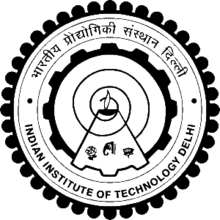
\includegraphics[width=4cm]{iitd_logo.png}
\end{figure}

\end{center}

\thispagestyle{empty}
\newpage
\begin{center}
\begin{large}
 \textbf{Certificate}
\end{large}
\end{center}
This is to certify that the work contained in this project entitled "\textbf{Universal Quantum Computation using Discrete Time Quantum Walk} submitted by \textbf{Mukesh Bhati(Entry No:2013MT60604)}\\to Department of Mathematics,Indian Institute of Technology Delhi towards the requirement of degree \textbf{Integrated Masters in Mathematics and Computing} has been carried by him under my supervision.\\



\vspace{20 mm}
New Delhi-110016\hspace{160 pt}Dr. N. Shravan Kumar\\
\hspace*{20 pt} July 2018\hspace{210 pt}Project Supervisor

\thispagestyle{empty}

\newpage
\begin{center}
\begin{large}
 \textbf{Acknowledgements}
\end{large}
\end{center}
I would like to take this opportunity to express my deepest and sincere gratitude to my thesis supervisor \textbf{Dr. N. Shravan Kumar} for his valuable suggestions,discussions and continuous support throughout the course of the project.\\

I would also like to thank \textbf{Dr. Amit Priyadarshi} and \textbf{ Dr. Sivanandan Sampath} for guiding me throughout the project.

\newpage
\tableofcontents

\newpage
\begin{abstract}

{Quantum Computing is quickly growing research field. Quantum Computing use Quantum Mechanics fundamentals to perform tasks with the potential to achieve quadratic speed up over classical computation. there are many quantum algorithm purposed that works faster than classical one.\\

This thesis discussed Classical Random walk and Quantum Random walk with their applications. Also we have discussed how quantum walk can be used for quantum computation}
 
\end{abstract}

\newpage
\begin{center}
\begin{LARGE}
\textbf{I. Quantum Computation}
\end{LARGE}
\end{center}
\thispagestyle{empty}
\section{Introduction}
The aim of the project is to study and Analysis of different modules used in quantum computation. Then study of discrete time quantum walk and it's application in universal quantum computation. Our aim will be provide a mapping from circuit model to graphical model on which DTQW propagates.     
 \\

\subsection{What is Quantum Computing/Computers ?}
What is quantum computing? It's something that could have been thought up a long time ago. For any physical theory one can ask: what sort of machines will do useful computation? or, what sort of processes will count as useful computational acts? Alan Turing thought about this in 1936 with regard (implicitly) to classical mechanics, and gave the world the paradigm classical computer: the Turing machine. But even in 1936 classical mechanics was known to be false. Work is now under way in seeing what quantum mechanics means for computers and computing.

Quantum computation can be defined as the study of information processing tasks accomplished using quantum mechanical systems. It is a beautiful combination of quantum physics, computer science, and information theory(includes the foundations of both computer science and communications). This is without doubt one of the hottest topics at the current frontiers of
computing and one of the most striking aspects of it is the complete uncertainty about its future.It could rise to meet the expectations of enthusiasts of the field.In such a case, quantum computers will substantially impact our everyday life.


\subsection{Why Quantum Computing/Computers ?}
Quantum Computing/Computers works safer and faster for certain kind of problems than classical computers. Many quantum algorithm are developed that computes faster than classical one. Database search algorithm that can be done using Grover's algorithm having time complexity $O(\sqrt{n})$, gives quadratic speed over classical algorithms.

According to moore's law computer's double every 18th months. Once quantum computers comes into pictures this may end. N-Qubit quantum computer store $2^n$ classical bits. so for large N this may be large number. There are many very good reasons for exploring quantum computing as much as possible.
\begin{itemize}
\item Making use of quantum effects allows one to speed-up certain computations enormously and even enables some things that are impossible for classical computers
\item The process of miniaturization that has made current classical computers so powerful and cheap, has already reached micro-levels where quantum effects occur. Chip-makers tend to go to great lengths to suppress those quantum effects, but instead one might also try to make good use of them.
\end{itemize}

\subsection{Differences between the classical and quantum information processing?}
Classical Information can be read and duplicated. where as quantum computation can not be read in general and can nor be duplicated, but it can be \textbf{teleported}.

The main difference is that quantum information has a special phenomena—called \textbf{Entanglement} which is not available in classical case. This allows that quantum information can be encoded in mutual correlations between remote parts of physical systems.

\section{From Randomized to Quantum Computation}
Comparing Quantum Turing Machine(QTM) to Probabilistic Turing machines(PTM) allows us to find out the difference between basic models of quantum and classical computing. 

\subsection{Probabilistic Turing Machines}
\textbf{probabilistic Turing machine}, having the finite alphabet $\sum$ and a finite set Q of states, is given by a transition function
\begin{center}
$\delta = \sum \times Q \times \sum \times Q \times \{\leftarrow,\downarrow,\rightarrow\} \longrightarrow [0,1]$
\end{center}
meaning that it assign a probability to each possible transition in such a way that the configuration
$c_0$ and all its successor-configurations $c_i$ the local probability condition is satisfied. if $p_i$ is transition probability from $c_0$ to $c_i$ then
\begin{center}
$\sum_{i=1}^{k}p_i = 1$
\end{center}
It is true that if a PTM satisfies all local probability conditions, then it also satisfies
all global probability conditions.

\subsection{Quantum Turing Machines}
Formally, a (one-tape) \textbf{quantum Turing machine}, on a finite set Q of states and the
finite alphabet $\sum$, is given by a transition function
\begin{center}
$\delta = \sum \times Q \times \sum \times Q \times \{\leftarrow,\downarrow,\rightarrow\} \longrightarrow \mathbb{C}_[0,1]$
\end{center}
assigning to each possible transition a probability amplitude in such a way that for each configuration
$c_0$ and all its successor-configurations $c_1, . . ., c_k$ the following local probability condition is satisfied
\begin{center}
$\sum_{i=1}^{k}\left|\alpha_i\right |^2 = 1$
\end{center}
where $\alpha_i$ is transition amplitude from $c_0$ to $c_i$.\newline
It is not true that if a QTM satisfies all local probability conditions, then it also satisfies
all global probability conditions.


\section{Introduction to quantum mechanics}
Quantum mechanics is a mathematical framework or set of rules for the construction of physical theories.
\subsection{ Linear Algebra in Dirac’s Notation}
Dirac’s bra/ket notation is used throughout quantum physics to represent quantum states and their transformations. In Dirac’s notation, a ket such as $\ket{v}$ corresponds to a column vector v, where v is an arbitrary label, refers to a vector representing a state of a quantum system so
\begin{align}
    \ket{v} &= \begin{pmatrix}
           a_{1} \\
           a_{2} \\
           \vdots \\
           a_{m}
         \end{pmatrix}
  \end{align}
In Dirac’s notation, the conjugate transpose of a ket $\ket{v}$ is called a bra and is written $\bra{v}$, so
\begin{align}
\bra{v} &= \begin{pmatrix}
           \conjugatet{a_{1}} & \conjugatet{a_{2}} & \hdots \conjugatet{a_{m}}
         \end{pmatrix}
\end{align}

\subsubsection{Inner Products}

The standard inner product $\braket{a}{b}$ is defined by a function $(.,.)$ from $V \cross V $ to $\mathbb{C}$ which satisfies:\\
1. $(.,.)$ is linear in second argument,
\begin{center}
    $(\ket{a, \sum_{i} C_i \ket{b_i}}) = \sum_{i}C_{i}(\ket{a},\ket{b_i})$
\end{center}
2. $(\ket{a},\ket{b}) = (\ket{b},\ket{a})^*$.\\
3. $(\ket{a},\ket{a}) \geq 0$.\\
4. $(\ket{a},\ket{a}) = 0 \iff \ket{a} =0$

For example, a inner product on $\mathbb{C}$ can be defined by multiplying the conjugate transpose $\bra{a}$= \begin{pmatrix}
    $\conjugatet{a_{1}} & \conjugatet{a_{2}}&\hdots \conjugatet{a_{m}}$
\end{pmatrix} with $\ket{b}$:

\braket{a}{b} = $\bra{a}$ $\ket{b}$ =  
\begin{pmatrix}
    \conjugatet{a_{1}} & \conjugatet{a_{2}} & \hdots \conjugatet{a_{m}} 
\end{pmatrix}
\begin{pmatrix}
           b_{1} \\
           b_{2} \\
           \vdots \\
           b_{m}
         \end{pmatrix}
=\sum_{i=1}^{n}\conjugatet{a_i} b_i.

Dirac’s choice of bra and ket arose as a play on words: an inner product $\braket{a}{b}$ of a bra $\bra{a}$ and a ket $\ket{b}$ is sometimes called a bracket.


A vector $\ket{v}$ can be written as a linear combination of vectors $\ket{s_1}, \ket{s_2}, . . . , \ket{s_n}$ ($\ket{s_i}$ known as basis vectors). If there exist complex numbers $a_i$ such that
\begin{center}
$\ket{v} = a_1\ket{s_1}+a_2\ket{s_2}+$ ··· $+a_n\ket{s_n}$. 
\end{center}
Given a set of vectors S, the subspace of all linear combinations of vectors in S is called the span of S and is denoted span(S). A set of vectors B for which every element of V can be written uniquely as a linear combination of vectors in B is called a basis for V.\newline
In quantum mechanics, bases are usually required to be orthonormal.Two vectors $\ket{v_1}$ and $\ket{v_2}$ are said to be orthogonal if $\braket{v_1}{v_2} = 0$. A set of vectors is orthogonal if all of its members are orthogonal to each other.A set of vectors is said to be orthonormal if all of its elements are of length one and orthogonal to each other: a set of vectors $B = {\ket{\beta_1},\ket{\beta_2}, ... ,\ket{\beta_n}}$ is orthonormal if $\braket{\beta_i}{\beta_j} = \delta_i_j$ for all i,j where
\[ 
\delta_i_j=     \begin{cases} 
                    1 & $if i=j$\\
                    0 & otherwise
                \end{cases}
\]
\textbf{Inner Product Space:} A vector space equipped with an inner product.\\
\textbf{Hilbert Space:} A complete inner product space is known as Hilbert space.\\

In quantum mechanics we are mainly concerned Hilbert spaces, so whenever we say space we mean Hilbert space.\\

\subsubsection{Tensor Products in Hilbert spaces}
Suppose V and W are two Hilbert spaces with bases $B_1 = \{\ket{\alpha_1}, \ket{\alpha_2}, \hdots, \ket{\alpha_n}\}$ and $B_2 = \{\ket{\beta_1}, \ket{\beta_2},
\hdots , \ket{\beta_m}\}$ respectively. Then the tensor product $V \tens{} W$  
i an nm-dimensional vector space with a basis consisting of the nm elements of the form $\ket{\alpha_i} \tens{} \ket{\beta_j}$ where $\tens$ is the tensor product, an abstract binary operator that satisfies the following relations:\\
$(\ket{u} + \ket{v}) \tens{} \ket{w} =  \ket{u} \tens{} \ket{w} + \ket{v} \tens{} \ket{w}$ \\
$\ket{w} \tens{} (\ket{u} + \ket{v}) = \ket{w} \tens{}  \ket{u} + \ket{w} \tens{} \ket{v}$\\
$(a\ket{u}) \tens{} \ket{v} = \ket{u} \tens{} (a\ket{v}) = a(\ket{u} \tens{} \ket{v})$\\
Taking $k = min(n,m)$ , all elements of form $V \tens{} W$ have form\\
$\ket{v_1} \tens{}  \ket{w_1} + \ket{v_2} \tens{}  \ket{w_2} \hdots \ket{v_k} \tens{}  \ket{w_k}$ for some $\ket{v_i} \in V$ and $\ket{w_i} \in W$.
Moreover, all element can be written as
\begin{center}
$v = \sum c_{i,j}(\ket{\alpha_i}\tens{}\ket{\beta_j})$.
\end{center}

\subsubsection{Unitary Operators}
Computation takes place in quantum system through transformation from state space of a closed quantum system to itself. In Quantum system arbitrary transformations do not allowed. The operator used for transformation must respect quantum properties like measurements and super-positions. Also transformation must be linear with state space and should preserve the length of vectors. linearly means
\begin{center}
    $U(a_1\ket{\Phi_1} + a_2\ket{\Phi_2} + \hdots + a_n\ket{\Phi_n}) = a_{1}U\ket{\Phi_1} + \hdots + a_{n}U\ket{\Phi_n}$
\end{center}
 Moreover, first measuring in some basis and then applying a operator $U$ to the outcome should give the same result as first applying the operator $U$ and then measuring in the transformed basis. The above all properties satisfy if operator preserve inner product:
 \begin{center}
     $\bra{\Phi}U^{*}U\ket{\Psi} = \bra{\Phi}\ket{\Psi}$
 \end{center}
 To satisfy above all conditions unitary transformation comes into role. A transformation is called unitary if
\begin{center}
$U^{*}U=\mathbb{I}$
\end{center}
this mean its adjoint $U^{*}$ must be equal to its inverse.
\begin{itemize}
\item U is unitary if and only if the set of columns of its matrix representation are orthonormal.
\item similarly U is unitary if and only if the set of rows of its matrix representation are orthonormal.
\item  The tensor product $U_1 \tens{} U_2$ is a unitary transformation of the space $X_1 \tens{} X_2$ if $U_1$ and $U_2$ are unitary transformations of $X_1$ and $X_2$ respectively.
\end{itemize}



\section{The postulates of Quantum Mechanics}

\subsection{State Space}
Every isolated physical system has an associated complex vector space with inner product (Hilbert space) called as state space of system. The system's state is described by unit vector, which is known as state vector in system's state space.  

For a given physical system, Quantum mechanics does not tells that what state space is associated with there physical system and what are the state vectors in that state space. we make some assumptions for our propose about state space.\\
1. The most fundamental quantum system concern with qubit.\\
2. State space of qubit is Hilbert space $\mathbb{C}^2$.\\
3. $\ket{0}$ and $\ket{1}$ are orthonormal basis for state space. which we describe by $$\ket{0} = \begin{pmatrix}
           1 \\
           0
\end{pmatrix} \hspace{1cm} \ket{1} = \begin{pmatrix}
           0\\
           1
\end{pmatrix}$$
4. any arbitrary state $\ker{\phi}$ can be written as linear combination of basis states as $$\ket{\phi} = a\ket{0} + \ket{b}$$
where a and b are complex numbers.

\subsection{Evolution}
The time evolution of an isolated or closed quantum system is described by unitary transformation. let at time $t_1$ system is in state $\Phi_1$ and at time $t_2$ the state is $\ket{\Phi_2}$ then $\ket{\Phi_2}$ can be obtain from $\phi_1$ using unitary transformation as follows:
$$\ket{\Phi_2} = U \ket{\Phi_1}$$.
This untary transform preserve its norm. means, if $\Phi$ is a unit vector then $U\phi$ is also an unitary vector. The important unitary operators on a single qubit are:\\
\textbf{Pauli Matrices:} $$I = \begin{pmatrix}
           1 & 0\\
           0 & 1
\end{pmatrix} \hspace{1 cm} X = \begin{pmatrix}
           0 & 1\\
           1 & 0
\end{pmatrix}$$
$$Y = \begin{pmatrix}
           0 & \di\\
           \di & 0
\end{pmatrix} \hspace{1 cm} z = \begin{pmatrix}
           1 & 0\\
           0 & -1
\end{pmatrix}$$

This postulates describe how closed quantum system's quantum states at different times are related to each other. There is more refined version of this postulates whick describe evolution of a quantum system in continuous time using Schrodinger equation. It make use of Hermitian operator.

\subsection{Quantum Measurements}
Measurements is the amount of information that can be obtain about the state. Theoretically, a qubit can hold an infinite amount of information. However, we cannot extract more information from such a
qubit than we are able to do it from a classical bit. The reason is that we have to measure the qubit in order to determine which state it is in.

Quantum measurement are describe by a collections ${M_n}$ of measurement operator. These operators act on system state space to measure it. Let $\ket{\Phi}$ is the state before measurement then the probability that result m occurs is given by 
$$p(m) = \bra{\Phi|M^{*}M|\ket{\Phi}}$$,
and the state after measurement is given by 
$$ \dfrac{M_m \ket{\Phi}}{\sqrt{\bra{\Phi|M^{*}M|\ket{\Phi}}}}$$
also measurement operators satisfy following conditions,
$$\sum_{m}M_{m}^{*}M_{m} = \mathbb{I}$$.

\textbf{Motivation :} In Postulate 2, we told that quantum system evolve according to unitary evolution. But if an experimenter wants to take measurement with the some equipment then he has to interact with system. It means system is no longer remains closed and hence not subjected to unitary evolution. thus postulate 3 is introduce to tell us about impacts of these measurements on the system.

\subsection{Superposition}
Let some physical system that can be in N different, mutually exclusive classical states say $\ket{0},\ket{1} .... \ket{N}$. In a classic state mean a state in which the system
can be found if we observe it. but a quantum state can be a superposition
of classical states
\begin{center}
$\ket{\Phi} = \alpha_1\ket{0} + \alpha_2\ket{0}+ ..... +\alpha_N\ket{N} $
\end{center}
Here $\alpha_i$ is a complex number that is called the amplitude of $\ket{i}$ in $\ket{\Phi}$

Mathematically, the states $\ket{1}, ..... \ket{N}$ form an orthonormal basis of an N-dimensional Hilbert space of dimension N, and a
quantum state $\ket{\Phi}$ is a vector in this space.

\subsection{Composite System}
composite physical system's state space is the tensor product of the state space of component physical system. For example, Let $\ket{\phi}$ is the state of composite system having n components then $\ket{\phi}$ can be written as $\ket{\phi_1} \tens{} \ket{\phi_2} \tens{} \hdots \tens{} \ket{\phi_n}$.

This postulates is useful when we interested in a composite physical system made up by two or more distinct physical system.

\subsection{Entanglement}
A state of a composite system which can not be written as a tensor product of state of its component systems then it is known as entangled state. For Example,
$$\ket{\phi} = \dfrac{\ket{00} + \ket{11}}{\sqrt{2}}$$
This state can not be written as tensor product of any two single qubit states. This state is known as \textbf{Bell state or EPR pair}.

Entanglement state arise naturally as result of interaction of quantum systems. It plays very important role in quantum computation and quantum information.


\section{Quantum Computation}
In Quantum system quantum state changes can be described by the language of quantum computation. Just like classical computation have classical bits, registers, gates and networks as basic elements. similarly quantum computation have quantum bits, quantum registers, quantum gates and quantum networks basic elements that are very different from classical one. In this section we will learn about all these basic elements for computation.


\subsection{Quantum Bits and Registers}
The bit is the fundamental unit of information in which it is measured. Quantum bits or qubit is basic unit of quantum information. Quantum computation and Quantum information are built upon on this concept.
\subsubsection{Qubits}
Just like a classical bit has a state either 0 or 1, qubit also has state. but the difference is that qubit can have other than that. It can be written as linear combination of these basic states. In other words, Let S be a two-dimensional quantum system with two orthonormal states, denoted $\ket{0}$ and $\ket{1}$ that can be considered as forming a standard basis of S. \vspace{5mm} \newline
\textbf{Definition 3.1.1} A \textbf{qubit} is a quantum state 
\begin{center}
 $\ket{\Phi}$ = \alpha$\ket{0}$ + \beta$\ket{1}$
\end{center}
where $\alpha,\beta \in \mathbb{C}$ and $\left|\alpha\right |^2 + \left|\beta\right|^2 $ = 1.\newline

One way we can say that a qubit is a unit vector in two-dimensional inner-product space.for which a particular orthonormal basis, denoted by $\{\ket{0},\ket{1}\}$ has been fixed. So, This is the fundamental difference distinguishing quantum bits from classical ones and is a direct application of the quantum principle of superposition of states.\par
Apart from mathematical defination there are  real physical systems which
may be described in terms of qubits. Possible physical realizations of a qubit include two different polarizations of a photon, the alignment of a nuclear spin in a uniform magnetic field or two electronic levels in an atom.

Since qubit can take any quantum linear superposition of $\ket{0} and \ket{1}$. This means that a large, even infinite, amount of information could potentially be encoded in amplitudes of a single qubit by appropriately choosing $\alpha$ and $\beta$.\\
\\
\textbf{Qubit Measurement in computational basis :}
For an unknown state $\ket{\phi}$ of qubit it is impossible to identify fully by a projection measurement. More exactly, we can get information from a qubit via projection measurement as only one classical bit of information. So from the information theory point of view, we can obtain only exactly same amount of information as classical information via measurement, even if it has infinitely many potential states.

Measurement of single qubit comes have measurements operators:
$$M_0 = \ket{0}\bra{0} \hspace{1cm} M_1 = \ket{1}\bra{1}$$
Each measurement operators is Hermitian. Now suppose Qubit is in state $\ket{\phi} = \alpha\ket{0} + \beta\ket{1}$. Then the probability of obtaining outcomes 0 is
$$p(0) = \bra{\phi}M_0^{*}M_0\ket{\phi} =\bra{\phi}M_0\ket{\phi} = \left|\alpha\right |^2 $$
similarly $p(1) = \left|\beta\right|^2$. and State after measurement of 0 is:
$$\dfrac{M_0\ket{\phi}}{\left|\alpha\right |} = \dfrac{\alpha}{\left|\alpha\right |}\ket{0}$$.
hence post measurement state is $\ket{0}$. similarly if we were measuring with $M_1$ then post measurement state would have been $\ket{1}$.\\
\textbf{Qubit Measurement in bases other than computational basis :}
Let Qubit is in state $\ket{\phi} = \alpha\ket{0} + \beta\ket{1}$. Measurement basis are $\ket{+} = \dfrac{\ket{0}+\ket{1}}{\sqrt{2}}$ and $\ket{-} = \dfrac{\ket{0}-\ket{1}}{\sqrt{2}}$ then qubit state can be expressed in $\ket{+}$ and $\ket{-}$ as :
$$\ket{\phi} = \alpha\ket{0} + \beta\ket{1} = \alpha\dfrac{\ket{+}+\ket{-}}{\sqrt{2}} + \beta\dfrac{\ket{+}-\ket{-}}{\sqrt{2}} = \dfrac{\alpha+\beta}{\sqrt{2}}\ket{+} + \dfrac{\alpha-\beta}{\sqrt{2}}\ket{-}$$.
so in new basis we get $p(+) =\dfrac{\left|\alpha + \beta\right|^2 }{2}$ and $p(-) =\dfrac{\left|\alpha - \beta\right|^2 }{2}$

\subsubsection{Multiple Qubit System}
Now let us generalize from one qubit to multiple qubit. Suppose $V_i$ $(0 \leq i \leq n-1) $ be the vector spaces, with basis $\{\ket{0}_i,\ket{1}_i\}$, corresponding to a single qubit. The standard basis for the vector space $V = V_{n-1} \tens{} \hdots \tens{} V_1 \tens{} V_0$ for an n-qubit system consists of the $2^n$ vectors
\begin{center}
$\{\ket{0}_{n-1} \tens{} \hdots \tens{} \ket{0}_1 \tens{} \ket{0}_0,$\\
$\{\ket{0}_{n-1} \tens{} \hdots \tens{} \ket{0}_1 \tens{} \ket{1}_0,$\\
$\{\ket{0}_{n-1} \tens{} \hdots \tens{} \ket{1}_1 \tens{} \ket{0}_0,$\\
$\vdots$\\
$\{\ket{1}_{n-1} \tens{} \hdots \tens{} \ket{1}_1 \tens{} \ket{1}_0,$\\
\end{center}
an even more compact and readable notation uses $\ket{b_{n-1} \hdots b_0}$ to represent $\ket{b_{n-1}} \tens{} \hdots \tens{} \ket{b_0}$.Moreover, the standard basis for an n-qubit system is written $\{\ket{0},\ket{1},\ket{2},\hdots,\ket{{2^n}-1}\}$
\\
\\
\textbf{Projective Measurement in multiple Qubit system : }
projective measurement is described by a Hermitian operator O, called observable in the srate of the system being measured. which is diagnolizable as follows:
$$O = \sum \lambda P_{\lambda}$$ where $\lambda$ are eigenvalues and $P_{\lambda}$ are projectors to eigenspace associated to corresponding $\lambda$. 
For Example, Projector $P_k$ $(0\geq k \leq 2^n-1)$ in computational basis are defined as follows : $$P_k = \ket{k}\bra{k}$$
Projectors $P_1, . . . , P_k$  are pairwise orthogonal, meaning that $P_iP_j = 0$ if
$i \neq j$.
The projector $P_j$ projects on eigen space $V_j$ of the Hilbert space V , and every state
$\ket{\Phi} \in V$ can be decomposed in a unique way as $\ket{\Phi}= \sum_{j=1}^{m}\ket{\Phi_j}
 $ with $\ket{\Phi_j} = P_j\ket{\Phi} \in V_j$. Because the
projectors are orthogonal, the subspaces $V_j$ are orthogonal as well, as are the states $\ket{\Phi_j}$. When we
apply this measurement to the pure state $\ket{\Phi}$, then we will get outcome j with probability $\norm{\ket{\Phi}}^2 = Tr(P_j\ket{\Phi}\bra{\Phi}) $ and the state will then “collapse” to the new state $\ket{\Phi}/\norm{\ket{\Phi}}=P_j\ket{\Phi}/\norm{P_j\ket{\Phi}}$.

\subsubsection{No-Cloning theorem}
\textbf{Theorem 5.1.3.1 :} An unknown state can not be clone using any unitary transformation. Namely, there is no unitary transformation U, such that state $\ket{\phi}$, $U(\ket{\phi,0}) = \ket{\phi,\phi}$. No Cloning theorem hold for any Hilbert space.\\
\textbf{Proof :} Let assume that there exist such unitary transformation U and for two different orthogonal state $\ket{\phi}$ and $\ket{\psi}$, $U(\ket{\phi,0}) = \ket{\phi,\phi}$ and $\ket{\psi}$, $U(\ket{\psi,0}) = \ket{\psi,\psi}$. let $\ket{\gamma} = \dfrac{\ket{\phi} + \ket{\psi}}{\sqrt{2}}$. Then $U(\ket{\gamma,0}) = \dfrac{\ket{\phi,\phi} + \ket{\psi,\psi}}{\sqrt{2}} \neq \ket{\gamma,\gamma} = \dfrac{\ket{\phi,\phi} + \ket{\psi,\psi} + \ket{\phi,\psi} + \ket{\psi,\phi}}{2}$.

\subsection{Quantum Gates and Circuits}
Quantum circuits are the basic model used in quantum computation. Like as boolean gates and circuits are building blocks in classical computation, Quantum gates and quantum circuit which are quantum analogue of classical ones are natural elements used for quantum computation. Sequences of quantum gates are called quantum gate arrays or quantum circuits. In this section we will discuss about Gates and circuits.\\
\\
\textbf{Definition 5.2.1 :} A quantum gates with n inputs and n outputs is specified by a unitary operator $U: H_{2^n} \rightarrow H_{2^n}$ and it is represented by a unitary matrix of degree $2^n$.

\subsubsection{Quantum NOT Gate :}
It is a single qubit gate. Let a qubit is in state $\ket{\phi} = a\ket{0} + b\ket{1}$. it acts linearly and interchange the role of basic states, i.e. $a\ket{1} + b\ket{0}$.\\
The matrix notation of quantum NOT gate is given by :
$$X = \begin{pmatrix}
           0 & 1\\
           1 & 0
\end{pmatrix} $$
A quntum state $a\ket{0} + b\ket{1}$ can be written as following matrix notation:
$$\begin{pmatrix}
           a\\
           b
\end{pmatrix}$$
Applying NOT gate we get as follows:
$$ X \begin{pmatrix}
           a\\b
\end{pmatrix} = \begin{pmatrix}
           b\\a
\end{pmatrix}$$

\subsubsection{Condition for a matrix to be a Gate}
A Quantum Gate matrix should be a unitary matrix i.e. U is a Quantum Gate matrix if $U^*U = \mathbb{I}$ where $U^*$ is ad-joint of U. This condition arises because of the normalization condition.\\ 
By this constraint we can have many non-trivial quantum gates unlike classical gates. The following are two important Gates for computation.
$$Z = \begin{pmatrix}
           1 & 0\\
           0 & -1
\end{pmatrix}$$
The above gate lives $\ket{0}$ unchanged and flip the sign of other from $\ket{1}$ to $-\ket{1}$.\\
\textbf{Hadamard Gate :}
$$H = \dfrac{1}{\sqrt{2}}\begin{pmatrix}
           1 & 0\\
           0 & -1
\end{pmatrix}$$
This gate is sometimes describe as 'square-root of NOT' gate. Note that, $H^2 = \mathbb{I}$  thus applying twice H to a state does nothing to it.\\
The Following figure summarize the function of above described Gates:
\begin{figure}[htp]
    \centering
    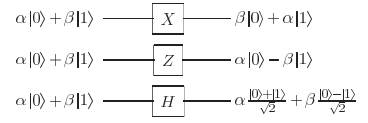
\includegraphics{Gates.png}
\end{figure}

\subsubsection{CNOT Gate}
One of the important Gate in multiple qubit gate is controlled-NOT or CNOT Gate. This gate takes input that control output, called as control qubit and other is target qubit. \\
This gate works as if control qubit is 0 then target gate remain same and if control qubit is 1 then it flip the target gate. the following way state transfer occur :
$$\ket{00} \rightarrow \ket{00}; \hspace{0.5cm}
\ket{01} \rightarrow \ket{01}; \hspace{0.5cm}
\ket{10} \rightarrow \ket{11}; \hspace{0.5cm}
\ket{11} \rightarrow \ket{10}$$
CNOT gate can be think as generalized version of XOR gate:
$$\ket{A,B} \rightarrow \ket{A, A\xor{B}}$$
Another way of describing is in matrix notation provided in figure below:
\begin{figure}[htp]
    \centering
    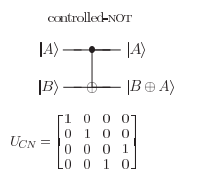
\includegraphics{CNOT.png}
\end{figure}

\subsubsection{Quantum Circuits}
Sequences of quan- tum gates are called quantum gate arrays or quantum circuits. Unlike many classical logic gates, quantum logic gates are reversible.\\
One of the example of quantum circuits is given in figure below. It takes two qubits and swap their state. Circuits are read from left to right.
\begin{figure}[htp]
    \centering
    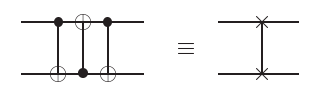
\includegraphics{Circuit.png}
\end{figure}\\
The operations performed by this circuit can be sequentially represented as:
$$\ket{a,b} \rightarrow \ket{a,a\xor{b}} \\
    \rightarrow \ket{a\xor{(a\xor{b})},a\xor{b}} = \ket{b,a\xor{b}}\\
    \rightarrow \ket{b,(a\xor{b})\xor{b}} = \ket{b,a}$$
\\

\newpage
\begin{center}
\begin{LARGE}
\textbf{II. Quantum Random Walks}
\end{LARGE}
\end{center}

Quantum walks can be considered as a quantum analogue of the classical random walk. It is most used in the development of quantum algorithms. Algorithm that are based on quantum walks use a technique called \textbf{amplitude amplification}, which is different from techniques used in algebraic algorithm. In this technique Fourier transform play an important role. There are many useful algorithms developed using quantum walk but element distinctness algorithm and Grover search algorithm are best ones. There are two classes of quantum walks, that is, the discrete-time and the continuous-time quantum walks.\\

Initially , we will briefly go through classical quantum random walks in which we will mainly focus on probability distribution and expected distance from the origin. further we will compare with quantum results. 

\section{Classical Random walk}
\subsection{Random walk on the Line}
The classical random walk in the line is the motion of a walker that lives the set of integers. The walker moves at each time step either one unit to th right with probability p or one unit left with probability 1-p. The directions of different steps are independent of each other and determined by non-biased coin. This classical random walks is known as Bernoulli random walk. Because this process is probabilistic, we cannot know for sure where the walker will be a later time. but we can calculate probability of being it in given state at time t. Following table describe the probabilities of walker in the positions 

\begin{center}
\begin{tabular}{ |c|c|c|c|c|c|c|c|c|c|c|c| } 
 \hline
 t / n   & -5 & -4 & -3 & -2 & -1 & 0 & 1 & 2 & 3 & 4 & 5 \\
 \hline
 0 &  &  &  &  &  & 1 &  &  &  &  &  \\
 \hline
 1 &  &  &  &  & 1/2 &  & 1/2 &  &  &  &  \\
 \hline
 2 &  &  &  & 1/4 &  & 1/2 &  & 1/4 &  &  &  \\
 \hline
 3 &  &  & 1/8 &  & 3/8 &  & 3/8 &  & 1/8 &  &  \\
 \hline
 4 &  & 1/16 &  & 1/4 &  & 3/8 &  & 1/4 &  & 1/16 &  \\
 \hline
 5 & 1/32 &  & 5/32 &  & 5/16 &  & 5/16 &  & 5/32 &  & 1/32 \\
 \hline
\end{tabular}
\end{center}
Figure : Probability of the walker being in the position n at time t, assuming it starts the random walk at the origin. The Probability is zero in empty cells.

\begin{figure}[htp]
\centering
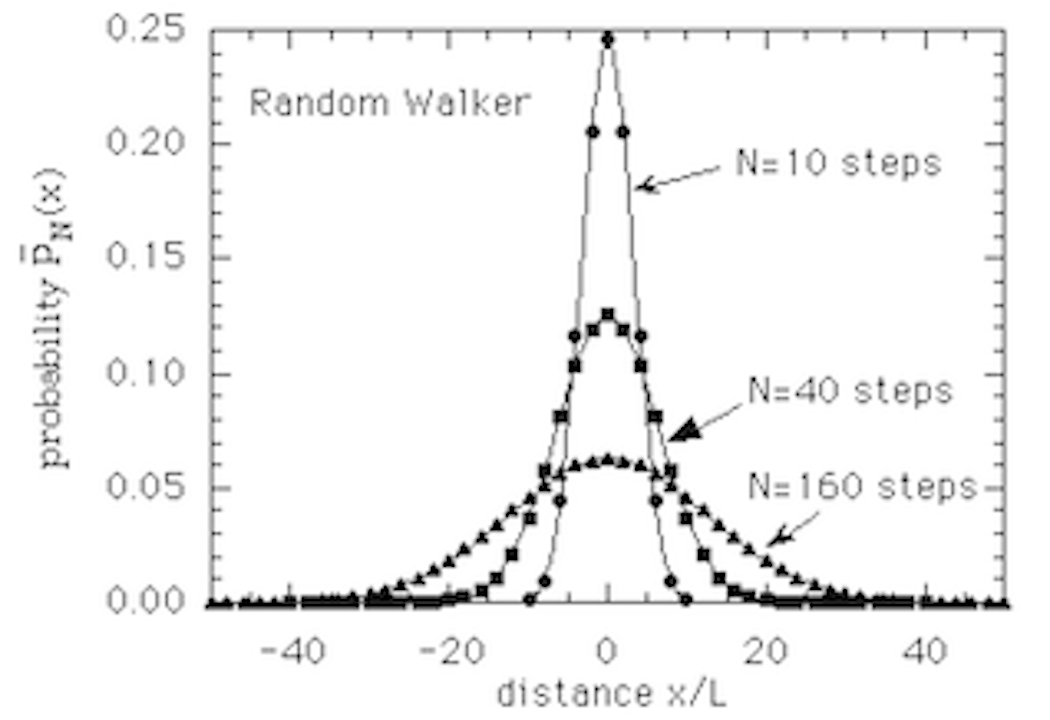
\includegraphics[width=10cm]{Classical_Probability.png}
\caption{Probability distribution of the random walk in a classical one-dimensional lattice for t= 10, t= 40 and t= 160}
\end{figure}
The above figure is for probability distribution of random walk in 1-D. From the curve we can observe that probability is zero for odd values of n when t is even. Another way to interpret the curve of the figure is as the sum $p(t,n) + p(t+1,n) $ i.e. we have two overlapping distributions.\\

There are few observations that can be seen in classical random walk. The first is probability distribution is symmetrical. Second is average position which is zero \\
\begin{center}
    $\mathbb{E}(n) = \sum_{n=-\infty}^{+\infty} np(t,n) = 0$
\end{center}

and standard deviation is 
\begin{center}
    $s.d = \sqrt{\mathbb{E}(n^2) -{\mathbb{E}(n)}^2} = \sqrt{t}$
\end{center}
Thus the variance varies linear with time steps. and also the probability distribution of the random walk can be approximated by the expression
\begin{center}
    $ p(t,n) \simeq \frac{2}{\sqrt{2\pi t}} e^{\frac{-n^{2}}{2t}}$
\end{center}

\section{Quantum Random Walks}
\subsection{Discrete Time Quantum Walk }
The quantum walk is a quantum generalization of the classical Bernoulli random walk. All the evolution is done by unitary operators acting on Hilbert space, whose size depends freedom of degree of associated physical system. In a quantum analogue of random walk, 'quantum coin' is used in place of classical coin which has basis states in state space.

The First model that we will discuss is the discrete time model. Simplest walk is one dimensional walk. In this walker can move on line of integers.
Now let us define the space of the system.

Hilbert space H of the system is defined by tensor product of the Hilbert spaces of the components i.e. $$H = H_{p} \tens{} H_{c}$$ 
where $H_{p} = $Position Hilbert space and $H_{c} = $ Coin Hilbert space.\\

In case of one dimension walk, computational basis of $H_{c}$ is $ \{\ket{0},\ket{1}\}$ and $H_{p}$ is $ \{\ket{n} : n\in \mathbb{Z} \}$. and the complete state of a walker is defined as follow:
$$\ket{\psi} = \sum_{n} \alpha_{n,1}\ket{n,1} + \alpha_{n,0}\ket{n,0}$$
For the coin state transfer we use is unitary operator which is called Coin Operator and then unitary conditional translation operator or shift operator which shift the state of walker corresponding the coin state. So in single step of a quantum walk involves a simultaneously application of coin operator followed by translation operator across all the states.
\\
\\
\textbf{Shift Operator}\\
The shift from $\ket{n}$ to $\ket{n+1}$ or $\ket{n-1}$ must be described by a unitary operator, called the shift operator S. It should operate as follow,
\begin{center}
    $ S \ket{0}\ket{n} = \ket{0} \ket{n+1}$
    $ S^* \ket{1}\ket{n} = \ket{1} \ket{n-1}$
\end{center}\\
So for above transformation we can define in following way
\begin{center}
    $S = \sum_{n \in \mathbb{Z}} \ket{n+1}\bra{n}$ and 
    $S^* = \sum_{n \in \mathbb{Z}} \ket{n-1}\bra{n}$
\end{center}
Applying Coin Operator C to initial state where C in unitary operator to determine the future state. Initial state of the coin can be one of the state of computational basis of $H_c$ but the result may be superposition of states. Let's start with $\ket{n=0}$ at origin state $\ket{0}$ Spin up. Now the initial state is $$\ket{\psi(0)} = \ket{0}\ket{n=0}$$ where $\ket{\psi(0)}$ denotes the initial state and $\ket{\psi(t)}$ denote the state at time t.
The coin used for most one-dimensional quantum quantum walk is the Hadamard operator $$ H = \dfrac{1}{\sqrt{2}}
\begin{pmatrix}
           1 & 1\
           1 & -1
\end{pmatrix}$$
$$ C  = H \tens{} I $$.
Now apply Hadamard operator on $\ket{0}$
$$H\ket{0}  = \dfrac{1}{\sqrt{2}}\begin{pmatrix}
           1 & 1\\
           1 & -1
\end{pmatrix} * \begin{pmatrix}
           1\\0
\end{pmatrix}$$
$$H\ket{0} = \dfrac{1}{\sqrt{2}}\begin{pmatrix}
           1\\1
\end{pmatrix}$$
and on $\ket{1}$
$$H\ket{1}  = \dfrac{1}{\sqrt{2}}\begin{pmatrix}
           1 & 1\\
           1 & -1
\end{pmatrix} * \begin{pmatrix}
           0\\1
\end{pmatrix}$$
$$H\ket{1} = -\dfrac{1}{\sqrt{2}}\begin{pmatrix}
           1\\1
\end{pmatrix}$$

Here er have sign difference but when we talk about probability of finding the walker at position the sign play no role. So here H is unbiased.\\
\\
\textbf{Quantum walk Unitary Operator}
\begin{center}
    $U = S ( H \tens{} I)$
\end{center}
where H is Hadamard coin, the most used coin in 1-D walk.\\
Appying U t times the state of quantum walk at time t is $$\ket{\psi(t)} = U^t\ket{\psi(0)}$$
Note: If we are given that at time t = 100 find the state of quantumwalk it is difficult so to make it simple we have simple method that will be discussed in later section.\\
\\
\textbf{Recursive formula based method:}\\
The generic state of the quantum walk can be written as a linear combination of the computational basis as
\begin{center}
    $\ket{\psi_n(x)} = \sum_{-\infty}^{\infty} (A_{x}(n)\ket{0} +(B_{x}(n)\ket{1}) \ket{x}$
\end{center}
where 
\begin{center}
    $ \sum_{-\infty}^{\infty} \abs{(A_{x}(n)}^2 + \abs{(B_{x}(n)}^2 = 1$
\end{center}
When applying $H \tens{} I $ followed by the shift operator, we can obtain recursive formulas involving the coefficients A and B, which are given by
\begin{center}
    $A_{x}(n+1) = \dfrac{A_{x-1}(n) + B_{x-1}(n)}{\sqrt{2}}$\\
    $B_{x}(n+1) = \dfrac{A_{x+1}(n) - B_{x+1}(n)}{\sqrt{2}}$
\end{center}
where initial condition is given by
\[ 
A_{x}(n)=     \begin{cases} 
                    1 & $if x=0$\\
                    0 & otherwise
                \end{cases}
\]
and $B_{x}(n)=0$.

Then we can easily find the probability distribution
$$ P(n,x) = \abs{(A_{x}(n)}^2 + \abs{(B_{x}(n)}^2 $$

\begin{figure}[htp]
    \centering
    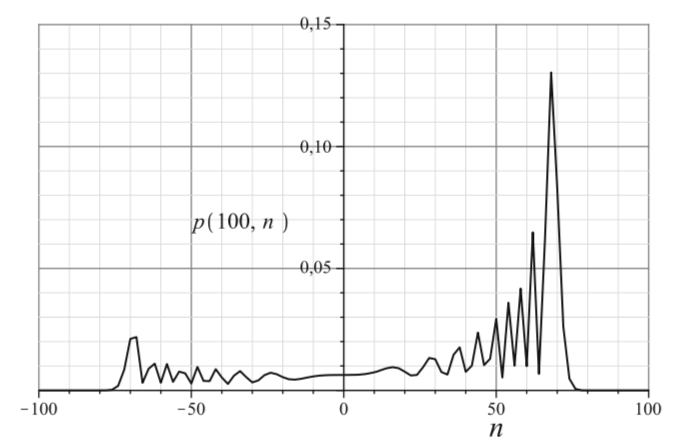
\includegraphics[width = 10cm]{Line_Graph.png}
    \caption{Probability distribution after 100 steps of a quantum walk with the Hadamard coin starting from the initial condition $\ket{\psi(0)} = \ket{0}\ket{n=0}$}
\end{figure}
By employing above method the graph in Fig 2 for the probability distribution after 100 steps will be obtained. In this we ignore null values of the probability. At t=100, the probability is zero for all odd values of n. The asymmetric probability distribution is evident. Probability of finding the walker on right side is larger than left side. This fact is valid for all values of t. This suggest the ballistic behaviour of the quantum walk. This behaviour can be due to the negative sign in hadamard coin which cause the cancellation of terms in left side movement. This can be confirm by the analysis using the initial condition $$\ket{\psi(0)} = -\ket{1}\ket{n=0}$$ 
In this case number of negative terms will be greater than positive terns. Thus the final result will be mirror image of Fig. 3 around vertical axis. So to obtain symmetric distribution, the initial must be superposition of these initial states. also superposition should not cancel the term before the probability calculation so we multiply with $\di$ with second initial condition. Hence initial condition :$$\ket{\psi(0)} = \dfrac{\ket{0}- \di\ket{1}}{\sqrt{2}}\ket{n=0}$$
Since the Hadamard coin have real entries so there will be no cancellation of terns of the walk. At the end we got following probability distribution   
\begin{figure}[htp]
    \centering
    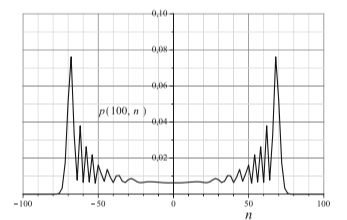
\includegraphics[width = 10cm]{Line_symmetric.png}
    \caption{Probability distribution after 100 steps of a quantum walk with the Hadamard coin starting from the initial condition $\ket{\psi(0)} = \dfrac{\ket{0}- \di\ket{1}}{\sqrt{2}}\ket{n=0}$}
\end{figure}

If the probability distribution of the quantum walk is symmetric, the expected position will be zero i.e $\ket{n=0}$. But below we will see that how standard deviation or expected distance from origin behaves with time. The formula for probability distribution is given by following way :
$$\sigma(t) = \sqrt{\sum_{n = -\infty}^{n=\infty}}n^{2}p(t,n)($$
where $p(t,n)$ is probability distribution.

\begin{figure}[htp]
    \centering
    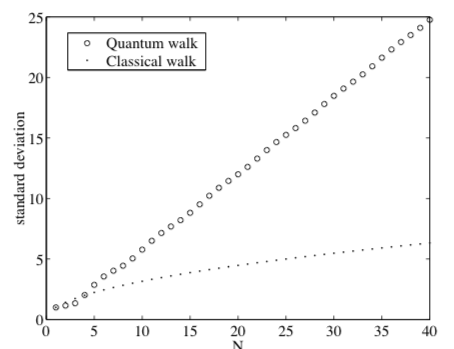
\includegraphics[width = 8cm]{Variance_Comp.png}
    \caption{Standard deviation of the quantum walk and classical random walk against number of steps}
\end{figure}

The Fig. 4 show the standard deviation as a function of time both the quantum walk and classical walk. In classical case $\sigma(t) = \sqrt{t}$ where as In quantum walk we obtain a line with slope around 0.54 i.e. $\sigma(t) = 0.54t$. This linear dependence play important role in quantum algorithm. However, the quantum walker can be found randomly on left side of origin or right side of origin. The quantum probability distribution is spread in the interval $[-\dfrac{t}{\sqrt{2}},\dfrac{t}{\sqrt{2}}]$, while the classical probability distribution is a Gaussian centered at the origin.  

\section{Quantum walk on Graphs}
This section present procedure for calculating analytic solution of quantum walks using Fourier transform on various geometries for example line, 2D-lattice, Cycle, Hyper-cube etc. Here are finite and infinite cases of graphs have been discussed.

\subsection{Discrete Time Quantum Walk on Infinite Graph}
Quantum walk on the line were introduced earlier in order to highlight some features which are strikingly different from the classical random walk. In this section, we will present detail analytic calculation of the quantum walk on the line. This calculation is a model for the study of quantum walks on many types of graphs. The Fourier transformation is key to success to this calculation.

We also analyze quantum walk on the two dimensional infinite lattice. Since the evolution equations are very complex in this case, the analysis is performed numerically.

On infinite graphs, the quantum walk spreads indefinitely. One of the most interesting physical properties is the expected distance from the origin, which is measured by the standard deviation of the probability distribution.

\subsubsection{Quantum walk on Line}
Lets take an integer line for the movement of quantum walk, where the integer line has an associated Hilbert space $H_p$ of infinite dimension. So, Computational basis of $H_p$ is $$\{\ket{n}: n \in Z\}$$.
Here each element $\ket{n}$ represents a vertex on the line graph. and coin space is associated with $H_c$ with dimension 2 with computational basis
$$\{\ket{0},\ket{1}\}$$.
So, Hilbert space of the system is the tensor product of the both coin space and position space, which can be defined as $$H_c \tens{} H_p$$
with computational basis $$\{\ket{s,n}, s \in {0,1}, n \in Z\}$$
where spin up s = 0(moving rightward), s = 1 spin down(moving leftward).

The generic state at time t $$\ket{\psi(t)} = \sum_{s=0}^{1}\sum_{n=-\infty}^{n=\infty}\ket{\psi_{s,t}(t)\ket{s,n}}$$
Here $\ket{\psi_{s,t}(t)}$ are probability amplitudes such that 
$$\sum_{n=-\infty}^{n=\infty}|\ket{\psi_{0,t}(t)}|^2 + |\ket{\psi_{1,t}(t)}|^2 \hspace{1cm}\forall t $$
The probability distribution is given by
$$P_n(t) = |\ket{\psi_{0,n}(t)}|^2 + |\ket{\psi_{1,n}(t)}|^2 $$
It is the probability of finding walker at $n^{th}$ vertex after t steps\\
\\
\textbf{Coin Operator}\\
Since degree of coin space is 2, Hadamard coin operator , which is given by $$H  = \dfrac{1}{\sqrt{2}}\begin{pmatrix}
           1 & 1\\
           1 & -1
\end{pmatrix}$$
Remember there are many other coins, choice depends in the performance. We will discuss later on the performance of various coins.
\\
\\
\textbf{Shift Operator}\\
After applying the coin operator we have to shift the position of walker accordingly. Shift Operator is defined by 
$$ S = \sum_{s=0}^{1}\sum_{n=-\infty}^{n=\infty} \ket{s,n+(-1)^s}\ket{s.n}$$
I mean, if s = 0, move the walker forward otherwise ,move it backward.
\\
\\
\textbf{Evolution Operator}\\
So, each step of the walk is defined by an Evolution operator. We have to apply this Evolution Operator to move state $\ket{\psi(t)}$ to $\ket{\psi(t+!}$ . The Standard evolution operator is defined by 
$$U = S(C\tens{}I)$$
When we apply the operator U on $t^{th}$ state, we get $(t+1)^{th}$ state as following
$$\ket{\psi(t+1)} = \sum_{n}S(\psi_{0,n}H\ket{0}\ket{n}+\psi_{1,n}H\ket{1}\ket{n})$$
After solving above we get following Walker's evolution equation
$$\psi_{0,n}(t+1) = \dfrac{\psi_{0,n-1}(t) + \psi_{1,n-1}(t)}{\sqrt{2}}$$
    $$\psi_{1,n}(t+1) = \dfrac{\psi_{0,n+1}(t) - \psi_{1,n+1}(t)}{\sqrt{2}}$$

These Equations can be solved using numerical simulations, but they are not that easy to do so. There is another way to obtain these evolution equations in different form, which are easy to calculate. For that we have to convert our computational basis to Fourier Basis that helps in diagonalizing the shift operator, eventually in diagonalizing the evolution operator.\\
\\ 
\textbf{Fourier Transform :}
The Fourier transformation of a discrete function $ f : \mathbb{Z} \rightarrow \mathbb{C}$ is a continuous function $\hat{f}: [-\pi,\pi] \rightarrow \mathbb{C}$ defined by
$$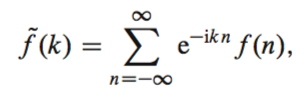
\includegraphics[width = 4cm]{FF.png}$$  
and the inverse transform is given by
$$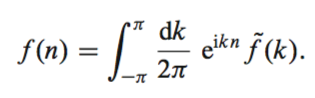
\includegraphics[width = 4cm]{IF.png}$$

The amplitudes $\ket{\psi_{s,n}(t)}$ discussed in previous section are discrete functions in variable n. Now we can above Fourier transform to calculate the Fourier transform to these amplitudes with respect to the variable n as follows:
$$\hat{\psi_{s}}(k,t) = \sum_{n}e^{\{-\di kn\}}\psi_{s,n}(t)$$
where $k \in [-\pi,\pi]$ is continuous.\\

As we have seen Walker's Evolution Equations for amplitudes, here we have to obtain Evolution Equations for $\hat{\psi_{s}}(k,t)$. If we are able to get these Evolution Equations for $\hat{\psi_{s}}(k,t)$ we can use Inverse Transform to obtain original Evolution Equations for $\psi_{s}(k,t)$.

Instead of transforming function $ f : \mathbb{Z} \rightarrow \mathbb{C}$, we transform the computational basis of $H_p$ So, our new basis is  
$$\{\ket{k_k} : -\pi \leq k \leq \pi\}$$
which canbe called as Fourier Basis. Where $$\ket{k_k} =  \sum_{n}e^{\{-\di kn\}}\ket{n}$$
Using this Fourier basis, we can represent the state of the quantum walker at time t as $$\ket{\psi(t)} = \int_{-\pi}^{\pi}\dfrac{dk}{2\pi}\sum_{s=0}^{1}\hat{\psi_{s}}(k,t)\ket{s}\ket{k_k}$$
Now apply the shift operator on the new Fourier basis, $\ket{s}\ket{k_k}$ and the definition of S we have
$$S\ket{s}\ket{k_k} = \sum_{n}e^{\di kn}S\ket{s,n}$$
$$S\ket{s}\ket{k_k} = \sum_{n}e^{\di kn}S\ket{s,n + (-1)^s}$$
lets substitute $n^{'} = n + (-1)^s$,
$$S\ket{s}\ket{k_k} = \sum_{n}e^{\di k(n^{'}-(-1)^s)}\ket{s,n^{'}} = e^{-\di k((-1)^s)}\ket{s}\ket{k_k}$$
above equations says that, shift operator only change its phase. $\ket{s}\ket{k_k}$ is an eigenvector of S, with eigenvalue $e{-\di k((-1)^s)}$. Using this, we have to find the eigenvectors of U, since out aim was to diagonalize U which gives analytics solution for amplitude equations.

Now apply U to $\ket{k_k}\ket{s^{'}}$
$$U\ket{k_k}\ket{s^{'}} = S \big\( \sum_{s=1}^{1}H_{s,s^{'}}\ket{k_k}\ket{s} =  \sum_{s=1}^{1}e^{-\di k((-1)^s)}H_{s,s^{'}}\ket{s}\ket{k_k}$$
Components of Evolution operator in the new basis are
$$\braket{s,k|U|s^{'},k_{k}^{'}} = e^{-\di k((-1)^s)}H_{s,s^{'}} \delta_{s,s^'}$$
$$\hat{H}_{s,s^{'}} = e^{-\di k((-1)^s)}H_{s,s^{'}}$$
Matrix of this can be represented as
$$\hat{H}_k = \begin{pmatrix}
           e^{-\di k} & 0\\
           0 & e^{\di k}
\end{pmatrix}*H$$
$$\hat{H}_k = \begin{pmatrix}
           e^{-\di k} & e^{-\di k}\\
           e^{\di k} & -e^{\di k}
\end{pmatrix}$$
So above equation reduces to 
$$U\ket{k_k}\ket{s} = (\hat{H}_k\ket{s})\ket{k_k}$$
If $\ket{\alpha_k}$ is an eigenvector of $\hat{H}_k$ with eigenvalue $\alpha_k$,
$$U\ket{k_k}\ket{\alpha_k} = (\hat{H}_k\ket{\alpha_k})\ket{k_k}$$
$$U\ket{k_k}\ket{\alpha_k} = \alpha\ket{\alpha_k}\ket{k_k}$$

Now it is enought to diagonalize $\hat{H}_k$ instead of diagonalising U. So the problem reduce from infinite dimension to 2-dimension. Now find characters-tic polynomial of $\hat{H}_k$ using
$$|\hat{H}_k - \lambda I| = 0$$
$$\lambda^2 + \di\lambda\sqrt{2}sin(k) -1 = 0$$
Roots or eigenvalues are 
$$\alpha_k = e^{-\di \omega_k}$$
$$\beta_k = e^{\di (\omega_k + \pi)}$$
where $\omega_k \in [\dfrac{-\pi}{2},\dfrac{\pi}{2}]$ such that $sin\omega_k = \dfrac{1}{\sqrt{2}}sin k$\\
\\
Now normalize the eigenvectors as follows:
$$\ket{\alpha_k} = \dfrac{1}{\sqrt{c^{-}}}\begin{pmatrix}
           e^{-\di k}\\
           \sqrt{2}e^{-\di \omega_k} - e^{-\di k}
\end{pmatrix}$$
$$\ket{\beta_k} = \dfrac{1}{\sqrt{c^{+}}}\begin{pmatrix}
           e^{-\di k}\\
           -\sqrt{2}e^{-\di \omega_k} - e^{-\di k}
\end{pmatrix}$$
where $C^{\rpm} = 2(1+cos^2 k)\rpm 2cosk\sqrt{(1+cos^2 k)}$.\\
\\
The spectral decomposition of Evolution operator U is given by
$$U = \int_{-\pi}^{\pi}\dfrac{dk}{2\pi}(e^{-\di\omega_k}\ket{\alpha_k}\ket{k_k}\bra{\alpha_k}\bra{k_k} + e^{\di(\omega_k+\pi)}\ket{\beta_k}\ket{k_k}\bra{\beta_k}\bra{k_k})$$

$$U^t = \int_{-\pi}^{\pi}\dfrac{dk}{2\pi}(e^{-\di\omega_k t}\ket{\alpha_k}\ket{k_k}\bra{\alpha_k}\bra{k_k} + e^{\di t(\omega_k+\pi)}\ket{\beta_k}\ket{k_k}\bra{\beta_k}\bra{k_k})$$
\\
\textbf{Analytic solution }
Lets start with initial condition $$\ket{\psi(0)} = \ket{0}\ket{n=0}$$
after t-step state of the quantum walk can be obtain using spectral decomposition of operator U, as follows
$$\ket{\psi(t)} = U^t\ket{\psi(0)} = \int_{-\pi}^{\pi}\dfrac{dk}{2\pi}(e^{-\di\omega_k t}\ket{\alpha_k}\ket{k_k}\bra{\alpha_k}\bra{k_k}\ket{0,0} + e^{\di t(\omega_k+\pi)}\ket{\beta_k}\ket{k_k}\bra{\beta_k}\bra{k_k}\ket{0,0})$$
and $$\bra{\alpha_k}\bra{k_k}\ket{0,0} = \dfrac{e^{\di k}}{\sqrt{c^{-}}}$$
$$\bra{\beta_k}\bra{k_k}\ket{0,0} = \dfrac{e^{\di k}}{\sqrt{c^{+}}}$$
\\
This reduce to 

$$\ket{\psi(t)} = \int_{-\pi}^{\pi}\dfrac{dk}{2\pi}(\dfrac{e^{-\di(\omega_k  t-k)}}{\sqrt{c^{-}}}\ket{\alpha_k} + \dfrac{e^{\di(\pi t+\omega_k t+ k) k}}{\sqrt{c^{+}}}\ket{\beta_k})\ket{k_k}$$

$$\ket{\psi(t)} = \int_{-\pi}^{\pi}\dfrac{dk}{2\pi}(\dfrac{e^{-\di(\omega_k  t-k)}}{\sqrt{c^{-}}} \dfrac{1}{\sqrt{c^{-}}}\begin{pmatrix}
           e^{-\di k}\\
           \sqrt{2}e^{-\di \omega_k} - e^{-\di k}
\end{pmatrix} + \dfrac{e^{\di(\pi t+\omega_k t+ k) }}{\sqrt{c^{+}}}\dfrac{1}{\sqrt{c^{+}}}\begin{pmatrix}
           e^{-\di k}\\
           -\sqrt{2}e^{-\di \omega_k} - e^{-\di k}
\end{pmatrix})\ket{k_k}$$
\\
Now calculate $\hat{\psi}_s(k,t)$
$$\hat{\psi}_0 (k,t) = \dfrac{e^{-\di(\omega_k  t)}}{c^{-}} + \dfrac{e^{\di(\pi t+\omega_k t+ k) }}{c^{+}} $$

$$\hat{\psi}_1(k,t) = \dfrac{e^{-\di(\omega_k  t-k)}(\sqrt{2}e^{-\di \omega_k} - e^{-\di k})}{c^{-}} + \dfrac{e^{\di(\pi t+\omega_k t+ k)}(\sqrt{2}e^{\di \omega_k} + e^{-\di k})}{c^{+}}$$

To simplify expression, we use
$$\frac{1}{c^{\rpm}} = \dfrac{1}{2}(1\mp \dfrac{cosk}{\sqrt{1+cos^2k}})$$

and 
$$\sqrt{2} e^{\mp\di\omega_k} \pm e^{-\di k} = \dfrac{c^{\pm}}{2\sqrt{1+cos^2k}}$$

so finally 
$$ \Hat{\psi}_0(k,t) = \dfrac{1}{2}(1 + \dfrac{cosk}{\sqrt{1+cos^2k}}) e^{-\di\omega_k t} +\dfrac{(-1)^t}{2}(1 - \dfrac{cosk}{\sqrt{1+cos^2k}}) e^{\di\omega_k t} $$

$$\hat{\psi}_1(k,t) = \dfrac{e^{\di k}}{2\sqrt{1+cos^2k}}(e^{-\di\omega_k t} - (-1)^t e^{\di\omega_k t)$$

Now our original amplitudes are given by Inverse transfrom as follows
$$\psi_{s,n}(t) = \int_{-\pi}^{\pi}\dfrac{dk}{2\pi}e^{\di k}\hat{\psi}_s (k,t)$$
and we finally have
$$\psi_{0,n}(t) = \int_{-\pi}^{\pi}\dfrac{dk}{2\pi}(1 + \dfrac{cosk}{\sqrt{1+cos^2k}}) e^{-\di(\omega_kt-kn)}$$

$$\psi_{1,n}(t) = \int_{-\pi}^{\pi}\dfrac{dk}{2\pi}(\dfrac{e^{\di k}}{\sqrt{1+cos^2k}}) e^{-\di(\omega_kt-kn)}$$
when $n+t$ is even. otherwise they are zero.
$$  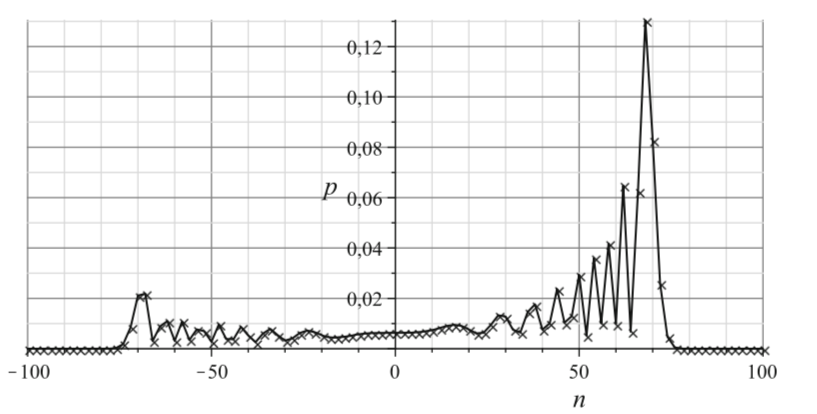
\includegraphics[width = 10cm]{PD_line.png}$$
Fig. Probability distribution of the quantum walk on the line after 100 steps from the analytical expression. The cross-shaped points correspond to integer values of n

\subsubsection{Quantum walk on 2-D lattice}
lets us take the 2-D lattice for the movement of quantum walk, with position space $H_p$ with computational basis ${\ket{x,y}: x,y \in \mathbb{Z}}$. Similar to 1-D problem, we can define new Hilbert space for the system which is $H_c \tens{} H_p$ where $H_c$ with computational basis 
$$\{\ket{i_x,i_y}: i_x,i_y \in \{0,1\} \}$$
The state of Quantum walker at time t is 
$$\ket{\psi(t)} = \sum_{i_x,i_y =0}^{1}\sum_{x,y}\psi_{{i_x,i_y};x,y}\ket{i_x,i_y}\ket{x,y}$$
The Probability distribution is
$$P_{x,y}(t) = \sum_{i_x,i_y =0}^{1}\sum_{x,y}|\psi_{{i_x,i_y};x,y}|^2$$
\\
\textbf{Shift Operator}
$$S\ket{i_x,i_y}\ket{x,y} = \ket{i_x,i_y}\ket{x+(-1)^{i}_{x},y + (-1)^{i}_{y}}$$
\\
\textbf{Evolution Operator}
$$U = S(C\tens{} I)$$
When we apply the operator U on $t^{th}$ state, we get next state as following

$$\ket{\psi(t+1)} = \sum_{i_x,i_y}^{1}\sum_{x,y}(\psi_{{i_x,i_y};x,y}S(C\ket{i_x,i_y}\ket{x,y})$$
$$\ket{\psi(t+1)} = \sum_{j_x,i_y}^{1}\sum_{x,y}(\psi_{{i_x,i_y};x,y}S(\sum_{i_x,i_y}^{1}C\ket{i_x,i_y}\ket{x,y})$$

$$ = \sum_{j_x,i_y}^{1}\sum_{x,y}(\psi_{{i_x,i_y};x,y}S(\sum_{i_x,i_y =0}^{1}C_{j_x,j_y;i_x,i_y}\ket{j_x,j_y}\ket{x,y})$$

$$ = \sum_{j_x,i_y}^{1}\sum_{x,y}(\psi_{{i_x,i_y};x,y}C_{j_x,j_y;i_x,i_y}\ket{i_x,i_y}\ket{x+(-1)^{i_{x}},y + (-1)^{i_{y}}}$$

substituting $x+(-1)^{i}_{x},y + (-1)^{i}_{y}$ to x,y
$$ \ket{\psi(t+1)} = \sum_{j_x,i_y}^{1}\sum_{x,y}\psi_{{i_x,i_y};x-(-1)^{i_{x}},y-(-1)^{i_{y}}}C_{j_x,j_y;i_x,i_y}\ket{i_x,i_y}\ket{x,y}$$

Now expanding left hand side in computational basis we get following evolution equantion
$$ \psi_{{i_x,i_y};x,y} = \sum_{j_x,i_y}^{1} \psi_{{i_x,i_y};x-(-1)^{i_{x}},y-(-1)^{i_{y}}}C_{j_x,j_y;i_x,i_y}$$
This equation is too complex to solve analytically for a generic coin. We will analyze the result for different coin.  
\\
\\
\textbf{The Hadamard Coin}\\
The hadamard coin is $C = H \tens{} H$ and its matrix representation is 
$$C = \dfrac{1}{2}\begin{pmatrix}
           1 & 1 & 1 & 1\\
           1 & -1 & 1 & -1\\
           1 & 1 & -1 & -1\\
           1 & -1 & -1 & 1\\
\end{pmatrix}$$
Let us take following state as initial state :
$$\ket{\psi(0)} = \dfrac{\ket{0}+\di\ket{1}}{\sqrt{2}} \tens{} \dfrac{\ket{0}+\di\ket{1}}{\sqrt{2}} \tens{} \ket{x=0,y=0}$$
We obtain symmetric Probability distribution for hadamard coin. The following fig. shows distribution
$$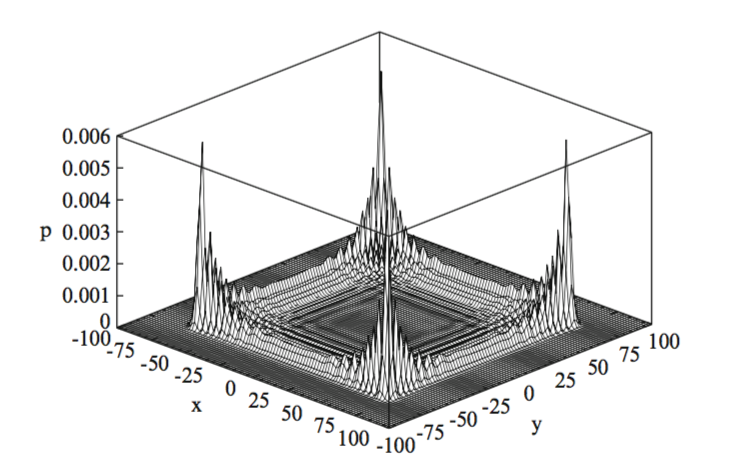
\includegraphics[width = 9cm]{Hadamard2D.png}$$
\textbf{The Fourier Coin}\\
The hadamard coin is $C = F_4$ and its matrix representation is 
$$C = \dfrac{1}{2}\begin{pmatrix}
           1 & 1 & 1 & 1\\
           1 & \di & -1 & -\di\\
           1 & -1 & 1 & -1\\
           1 & -\di & -1 & 1\\
\end{pmatrix}$$
Let us take following state as initial state :
$$\ket{\psi(0)} = \dfrac{1}{2}(\ket{00}+\dfrac{1-\di}{\sqrt{2}}\ket{01} + \ket{10}+ \dfrac{1-\di}{\sqrt{2}}\ket{11})\ket{x=0,y=0}$$
$$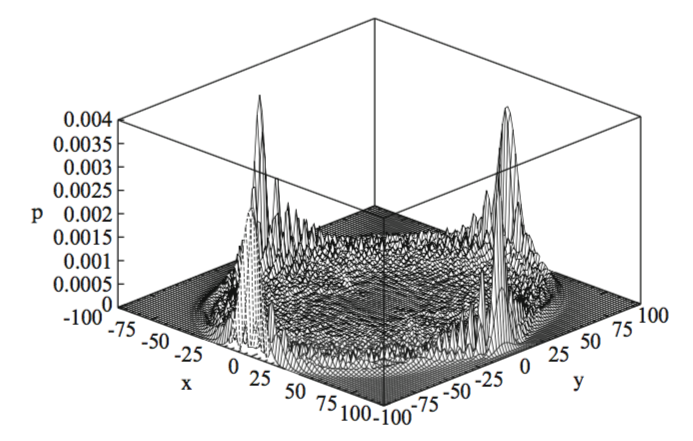
\includegraphics[width = 9cm]{Fourier2D.png}$$
\\
\textbf{The Grover Coin}\\
Finally, we will use the Grover coin which is given by
$$G = 2\ket{D}\bra{D} - I$$
where $$D = \dfrac{1}{2}\sum_{i_x,i_y}^{1}\ket{i_x,i_y=0}$$
The Matrix representation is
$$C = \dfrac{1}{2}\begin{pmatrix}
           -1 & 1 & 1 & 1\\
           1 & -1 & 1 & \\
           1 & 1 & -1 & 1\\
           1 & 1 & 1 & -1\\
\end{pmatrix}$$
The initial condition which has largest standard deviation for Grover coin is the state
$$\ket{\psi(0)} = \dfrac{1}{2}(\ket{00}-\ket{01} - \ket{10}+ +\ket{11})\ket{x=0,y=0}$$
$$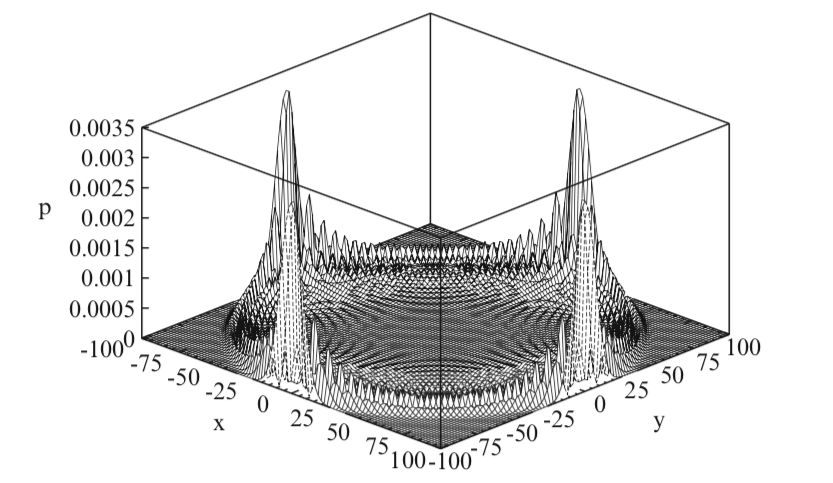
\includegraphics[width = 9cm]{Grover2D.png}$$
\\
\textbf{Comparison :} \\
\\To analysis the comparison between the coin we calculate standard deviation of the probability generated by each one. The following graph shows the standard deviation for all three coins
$$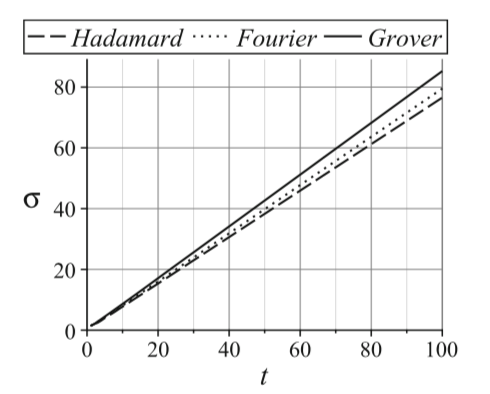
\includegraphics[width = 8cm]{Deviation.png}$$
From above graph we observe that Grover coin has largest standard deviation among the three coin. This lead to several advantage to Grover coin over other coins because this can be useful in algorithmic application. Grover coin can be used for any dimension where as Hadamard coin can be used only that are power of 2.

\subsection{Discrete Time Quantum walk on Finite Graph}
N-Cycle is a finite version of Line discussed in previous sections, such that if the walker moves N steps in any direction it reaches the initial point.

Position space has an associated Hilbert Space $H_p$ of dimension N. So, computational basis of $H_p$ is
$$\{\ket{j}, j\in \{0,\hdots, N-1\}\}$$
Coin space id associated with $H_c$ with dimension 2 with computational basis
$$\{\ket{0},\ket{1}\}$$
So, Hilbert space of the system is the tensor product of the coin space and position space.$$H^2\tens{}H^N$$
with computational basis $$\{\ket{s,j}, s\in\{0,1\}, j\in \{0,\hdots, N-1\}\}$$
\\
\textbf{Shift Operator}\\
\\
$$ S\ket{s.j} = \ket{s,j+(-1)^s}$$
To maintain its cycle property we need to consider j modulo N for every iteration.

The generic state at time t is describe by
$$\ket{\psi(t)} = \sum_{s=0}^{1}\sum_{j=0}^{j=N-1}\ket{\psi_{s,t}(t)\ket{s,j}}$$
such that
$$|\ket{\psi_{0,j}(t)}|^2 + |\ket{\psi_{1,j}(t)}|^2 \space \forall t$$
\\
\textbf{Coin Operator}
$$H  = \dfrac{1}{\sqrt{2}}\begin{pmatrix}
           1 & 1\\
           1 & -1
\end{pmatrix}$$
\\
\\
\textbf{Evolution Operator}\\
So, each step of the walk is defined by an Evolution operator. We have to apply this Evolution Operator to move state $\ket{\psi(t)}$ to $\ket{\psi(t+!}$ . The Standard evolution operator is defined by 
$$U = S(C\tens{}I)$$
When we apply the operator U on $t^{th}$ state, we get $(t+1)^{th}$ state as following
$$\ket{\psi(t+1)} = \sum_{j=0}^{N-1}S(\psi_{0,j}H\ket{0}\ket{j}+\psi_{1,j}H\ket{1}\ket{j})$$
After solving above we get following Walker's evolution equation
$$\psi_{0,j}(t+1) = \dfrac{\psi_{0,j-1}(t) + \psi_{1,j-1}(t)}{\sqrt{2}}$$
    $$\psi_{1,j}(t+1) = \dfrac{\psi_{0,j+1}(t) - \psi_{1,j+1}(t)}{\sqrt{2}}$$

These Equations can be solved using numerical simulations, but they are not that easy to do so. There is another way to obtain these evolution equations in different form, which are easy to calculate. For that we have to convert our computational basis to Fourier Basis that helps in diagonalizing the shift operator, eventually in diagonalizing the evolution operator.\\
\\ 
\textbf{Fourier Transform :}
To understand why do we need Fourier Transform, go through the Fourier Transform section Of Line in infinite graphs.\\

we get new basis is  
$$\{\ket{k_k} : 0 \leq k \leq N-1\}$$
which we called Fourier Basis. Where $$\ket{k_k} = \dfrac{1}{\sqrt{N}} \sum_{j=0}^{N-1}\omega_{N}^{jk}\ket{j}$$
and $$\omega_N = e^{\frac{2\pi\di}{N}}$$

Using this Fourier basis, we can represent the state of the quantum walker at time t as $$\ket{\psi(t)} = \sum_{s=0}^{1}\sum_{k=0}^{N-1}\hat{\psi_{s,k}}(t)\ket{s}\ket{k_k}$$
with the coefficient given by
$$\hat{\psi_{s,k}} = \dfrac{1}{\sqrt{N}} \sum_{j=0}^{N-1}\omega_{N}^{-jk}\psi_{s,j}$$
Now apply the shift operator on the new Fourier basis, $\ket{s}\ket{k_k}$ and the definition of S we have
$$S\ket{s}\ket{k_k} = \dfrac{1}{\sqrt{N}} \sum_{j=0}^{N-1}\omega_{N}^{jk}\ket{s,j}$$
$$S\ket{s}\ket{k_k} = \dfrac{1}{\sqrt{N}} \sum_{j=0}^{N-1}\omega_{N}^{jk}\ket{s,j + (-1)^s}$$
lets substitute $j^{'} = j + (-1)^s$,
$$S\ket{s}\ket{k_k} = \dfrac{1}{\sqrt{N}} \sum_{j=0}^{N-1}\omega_{N}^{k(j^{'}-(-1)^{s})}\ket{s,j^{'}} = \omega^{-k((-1)^s)}\ket{s}\ket{k_k}$$

above equations says that, shift operator only changing its phase. $\ket{s}\ket{k_k}$ is an eigenvector of S, with eigenvalue $\omega^{-k((-1)^s)}$. Using this, we have to find the eigenvectors of U, since out aim was to diagonalize U which gives analytics solution for amplitude equations.

Now apply U to $\ket{k_k}\ket{s^{'}}$
$$U\ket{k_k}\ket{s^{'}} = S \big\( \sum_{s=1}^{1}H_{s,s^{'}}\ket{k_k}\ket{s} =  \sum_{s=1}^{1}\omega^{-k((-1)^s)}H_{s,s^{'}}\ket{s}\ket{k_k}$$
Components of Evolution operator in the new basis are
$$\bra{s,k_k}U\ket{s^{'},k_{k}^{'}} = \omega^{-k((-1)^s)}H_{s,s^{'}} \delta_{k,k^'}$$
$$\hat{H}_{s,s^{'}} = \omega^{-k((-1)^s)}H_{s,s^{'}}$$
Matrix of this can be represented as
$$\hat{H}_k = \begin{pmatrix}
           \omega_{N}^{-k} & 0\\
           0 & \omega_{N}^{k}
\end{pmatrix}*H$$
$$\hat{H}_k = \begin{pmatrix}
           \omega_{N}^{-k} & \omega_{N}^{k}\\
           \omega_{N}^{k} & -\omega_{N}^{-k}
\end{pmatrix}$$
So above equation reduces to 
$$U\ket{k_k}\ket{s} = (\hat{H}_k\ket{s})\ket{k_k}$$
If $\ket{\alpha_k}$ is an eigenvector of $\hat{H}_k$ with eigenvalue $\alpha_k$,
$$U\ket{k_k}\ket{\alpha_k} = (\hat{H}_k\ket{\alpha_k})\ket{k_k}$$
$$U\ket{k_k}\ket{\alpha_k} = \alpha\ket{\alpha_k}\ket{k_k}$$

Now it is enought to diagonalize $\hat{H}_k$ instead of diagonalising U. So the problem reduce from infinite dimension to 2-dimension. Now find characters-tic polynomial of $\hat{H}_k$ using
$$|\hat{H}_k - \lambda I| = 0$$
$$\lambda^2 + \di\lambda\sqrt{2}sin(\dfrac{2\pi k}{N}) -1 = 0$$
Roots or eigenvalues are 
$$\alpha_k = e^{-\di \theta_k}$$
$$\beta_k = e^{\di (\theta_k + \pi)}$$
where $\theta_k \in [\dfrac{-\pi}{2},\dfrac{\pi}{2}]$ such that $sin\theta_k = \dfrac{1}{\sqrt{2}}\sin{\dfrac{2\pi k}{N}}$\\
Now normalize the eigenvectors as follows:
$$\ket{\alpha_k} = \dfrac{1}{\sqrt{c^{-}}}\begin{pmatrix}
           1\\
           (\sqrt{1+\cos^2({\dfrac{2\pi k}{N}})} - \cos^2{(\dfrac{2\pi k}{N})})e^{\di\dfrac{2\pi k}{N}}
\end{pmatrix}$$
$$\ket{\beta_k} = \dfrac{1}{\sqrt{c^{+}}}\begin{pmatrix}
           1\\
           -(\sqrt{1+\cos^2({\dfrac{2\pi k}{N}})} + \cos^2{(\dfrac{2\pi k}{N})})e^{\di\dfrac{2\pi k}{N}}
\end{pmatrix}$$
where $C^{\rpm} = 2\sqrt{1+\cos^2{(\dfrac{2\pi k}{N})} }(\sqrt{1+\cos^2({\dfrac{2\pi k}{N}})} \pm \cos^2{(\dfrac{2\pi k}{N})})$.
\\
\\
The spectral decomposition of Evolution operator U is given by
$$U = \sum_{k=0}^{N-1}(e^{-\di\theta_k}\ket{\alpha_k}\ket{k_k}\bra{\alpha_k}\bra{k_k} + e^{\di(\theta_k+\pi)}\ket{\beta_k}\ket{k_k}\bra{\beta_k}\bra{k_k})$$
after t time
$$U^t = \sum_{k=0}^{N-1}(e^{-\di\theta_k t}\ket{\alpha_k}\ket{k_k}\bra{\alpha_k}\bra{k_k} + e^{\di t(\theta_k+\pi)}\ket{\beta_k}\ket{k_k}\bra{\beta_k}\bra{k_k})$$
\\
\\
\textbf{Analytic solution }\\

Lets start with initial condition $$\ket{\psi(0)} = \ket{0}\ket{n=0}$$
after t-step state of the quantum walk can be obtain using spectral decomposition of operator U, as follows
$$\ket{\psi(t)} = U^t\ket{\psi(0)} = \sum_{k=0}^{N-1}(e^{-\di\theta_k t}\ket{\alpha_k}\ket{k_k}\bra{\alpha_k}\bra{k_k}\ket{0,0} + e^{\di t(\theta_k+\pi)}\ket{\beta_k}\ket{k_k}\bra{\beta_k}\bra{k_k}\ket{0,0})$$
and 
$$\bra{\alpha_k}\bra{k_k}\ket{0,0} = \dfrac{1}{\sqrt{Nc^{-}}}$$
$$\bra{\beta_k}\bra{k_k}\ket{0,0} = \dfrac{1}{\sqrt{Nc^{+}}}$$
\\
This reduce to 

$$\ket{\psi(t)} =  \dfrac{1}{\sqrt{N}}\sum_{k=0}^{N-1}(\dfrac{e^{-\di(\theta_k  t)}}{\sqrt{c^{-}}}\ket{\alpha_k} + \dfrac{e^{\di\theta_k t}}{\sqrt{c^{+}}}\ket{\beta_k})\ket{k_k}$$

To simplify expression, we use
$$\frac{1}{c^{\rpm}} = \dfrac{1}{2}(1\mp \dfrac{\cos{\hat{k}}}{\sqrt{1+\cos^2\hat{k}}})$$

$$\ket{\psi(t)} = \dfrac{1}{\sqrt{N}}\sum_{k=0}^{N-1}
\begin{pmatrix}
           A_k(t)\\
           B_k(t)
\end{pmatrix}\ket{k_k}$$
where
$$\hat{k} = \dfrac{2\pi k}{N}$$

$$A_k(t) = \cos{\theta_k t}- \dfrac{\di\cos{\hat{k}}\sin{\theta_k}t}{\sqrt{1+\cos^2(\hat{k})}}$$

$$B_k(t) = -\dfrac{\di e^{\di\hat{k}}\sin{\theta_k}t}{\sqrt{1+\cos^2(\hat{k})}}$$
Which is valid when t is even. we obtain
$$\ket{\psi(t)} = \dfrac{1}{\sqrt{N}}\sum_{j=0}^{N-1}
\begin{pmatrix}
           \sum_{k=0}^{N-1}A_k(t)e^{ij\hat{k}}\\
           \sum_{k=0}^{N-1}B_k(t)e^{ij\hat{k}}
\end{pmatrix}\ket{j}$$
We obtain the probability
$$p_j(t) = \dfrac{1}{N^2}|\sum_{k=0}^{N-1}A_k(t)e^{ij\hat{k}}|^2 + \dfrac{1}{N^2}|\sum_{k=0}^{N-1}B_k(t)e^{ij\hat{k}}|^2$$
This equation hold for any N, but only for even t. The following figure shows probability distribution of quantum walk on cycle.
$$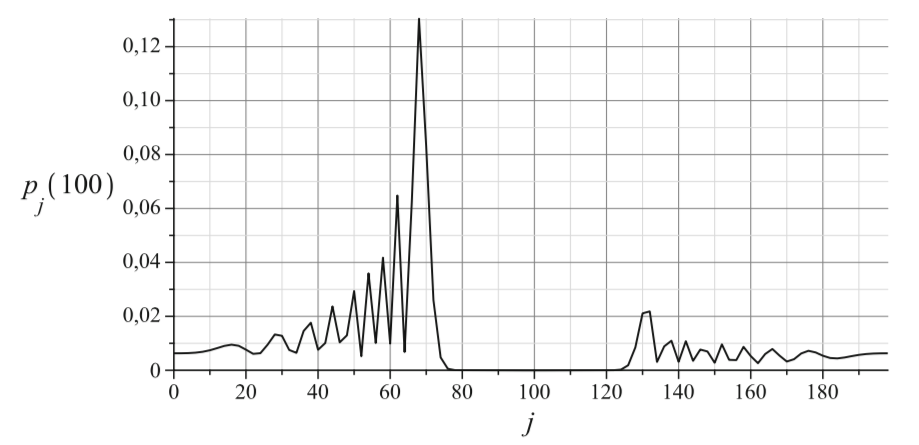
\includegraphics[width = 15cm]{Cycle.png}$$
\\
\\
\section{Universal Quantum Computation using Discrete Time Quantum Walk}
\subsection{Introduction}
In this section, we will see that how discrete time quantum walk can be used to implement the universal quantum gates. Universal quantum computation by continuous time quantum walk using unweighted graphs of low degrees was proposed by [6]Childs. This shows us university of Quantum walk. it means that any quantum algorithm can be recast as a quantum walk algorithm. An explicit construction that convert the quantum gates into a graph was initially presented by Childs. Later Lovett[] used same construction process but has maximum degree d, eight of any vertex as opposed to three in the continuous case. This construction require large graph size input, like for n qubit it require $2^n$ wires. Quantum computers need poly$\log(N)$ gates for N-size graph to simulates a Quantum graph.

Unlike continuous time quantum walk, in discrete time quantum walk we use a specific coin for no reflection at vertex in graph, to be move only in a direction. If we use $\sigma_x$, we restrict that any vertex can have only degree two, no way to construct higher degree graph. Thus, [] Lovett uses two edge wire to accomplish directional propagation. 

\subsection{Universal Gate Set}
Now in this section we will see how we can construct universal quantum gates using discrete time quantum walk. The standard universal gates are C-NOT gate,
$$C-NOT = \begin{pmatrix}
           1 & 0 & 0& 0\\
           0 & 1 & 0& 0\\
           0 & 0 & 0& 1\\
           0 & 0 & 1& 0\\
\end{pmatrix}$$
single qubit Hadamard gate,
$$H = \dfrac{1}{\sqrt{2}}\begin{pmatrix}
           1 & 1 \\
           1 & -1  
\end{pmatrix}$$
The phase shift gate
$$P(\dfrac{\pi}{8}) = \begin{pmatrix}
           1 & 0 \\
           0 & e^{\di\dfrac{\pi}{4}}  
\end{pmatrix}$$
These gates are known as universal gate set.\\

In construction for n qubit we need $2^n$ wires so, [6]Childs define  computational basis for quantum state as quantum wires. Then other gates can be constructed via quantum wire by connecting them. Then computation is done by quantum walk on these wire. 

Now we will see how to construct a simple wire, on which quantum walk propagated from input to output. Here []Lovett use two edge per wire for no reflection occur at the vertex. The walker then distributed across the edge with equal amplitude which combined at next vertex. at every vertex we use Grover coin that change input edges to output edges. Then we apply the shift operator to go next vertex. The following show the complete one step,
$$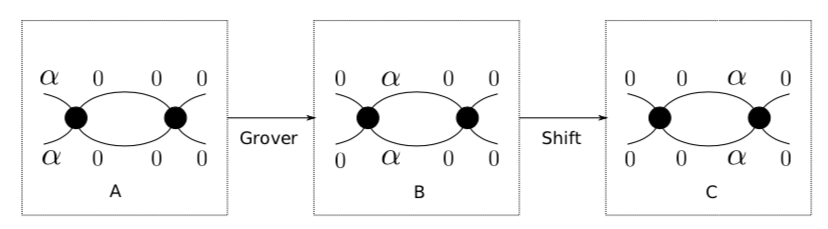
\includegraphics[width  = 15cm]{state_change.png}$$
\begin{center}
    Fig. 10.2 Grover coin and shift operation acting on vertex of degree d= 4.
\end{center}
The general Grover coin for any degree d is,
$$G^{(d)} = \begin{pmatrix}
           \dfrac{2}{d} & \hdots & \dfrac{2}{d}\\
           \vdots       & \ddots    &     \vdots\\
           \dfrac{2}{d} & \hdots  & \dfrac{2}{d}
\end{pmatrix} - I_{d}$$
The following Fig. show basic wire we use,
$$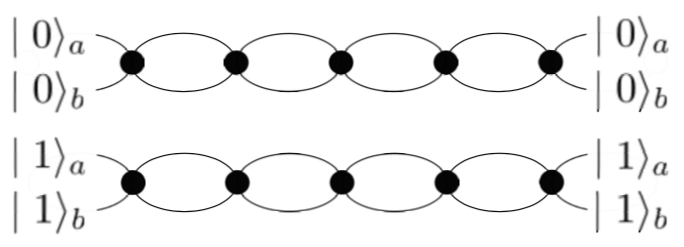
\includegraphics[width  = 12cm]{wire.png}$$
\begin{center}
    Fig. 10.3 The Basic wire used to propagates the quantum walk from left to right. Grover coin with $d=4$ is used.
\end{center}
The computation start with the amplitude at the initial vertex spread equally across the pair of edge in a wire. i.e. Let initial state $\ket{\psi} = \alpha\ket{0}+\beta\ket{1}$ where $\alpha$ and $\beta$ are complex numbers. it would split as follows,
$$\ket{\psi}_{initial} = \dfrac{1}{\sqrt{2}}(\alpha\ket{0}_a+\alpha\ket{0_b}+\beta\ket{1}_a+ \beta\ket{1}_b)$$
where a and b refer to the top line and bottom line of the wire respectively. The walk propagates from left to right on wire.

\subsubsection{C-NOT Gate}
It is trivial to implement C-NOT gate, just by exchanging the wire of single qubit. The following figure shows graphical C-NOT,
$$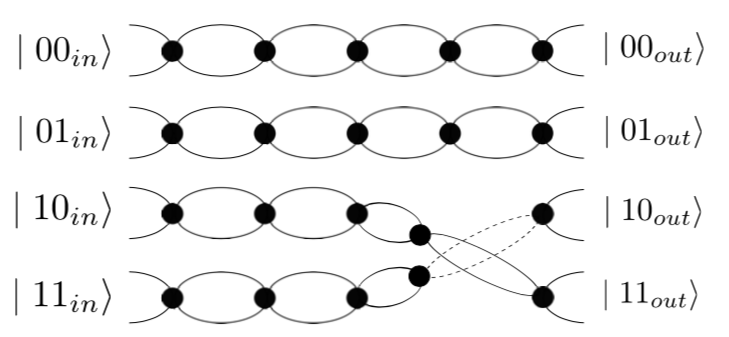
\includegraphics[width  = 12cm]{C-NOT.png}$$

\subsubsection{The Phase Gate}
In this Gate we require addition of relative phase to one wire related to other wire. To do this we make some changes to Grover coin as follow,
$$G_{\phi}^{(4)} = e^{\di\phi}G^{(4)}$$
This means at each vertex, the walk pick up a phase of $e^{\di\phi}$. So, For wire shown in fig. 10.3, walk would pick up a phase of $e^{5\di\phi}$ at the final vertex. The Phase Gate is given as follows,
$$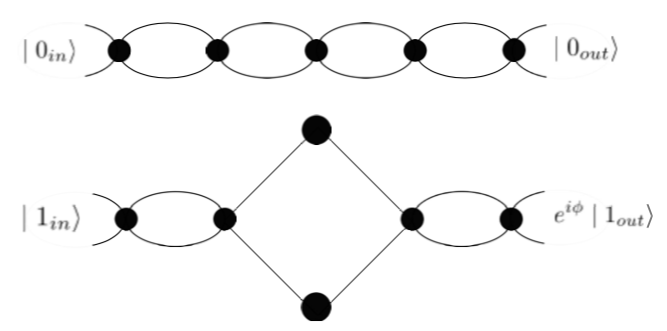
\includegraphics[width = 12cm]{Phase_Gate.png}$$
In the above structure there is vertex with degree d = 2, at which we use Grover coin with d = 2 with no phase added,
$$G^{(2)} = \begin{pmatrix}
           0 & 1\\
           1 & 0
\end{pmatrix}$$
So using above structure we get a phase Gate.

\subsubsection{Hadamard Gate}
This gate requires interaction between two basic wires (computational states). The following structure is used for hadamard gate,
$$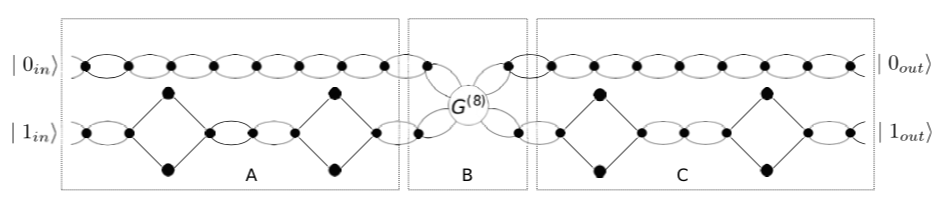
\includegraphics[width = 15cm]{Hadamard.png}$$
The above structure look little bit complex. To understand it, we divide it into parts A, B and C. Section A and C are used to get a relative phase $\di$ to wire $\ket{1}$ before and after B. And Section B is used to combine the wire $\ket{0}$ and $\ket{0}$, then split across output equally.
In this structure we have a vertex degree d = 8, for that we use Grover Coin $G^{(8)}$,
$$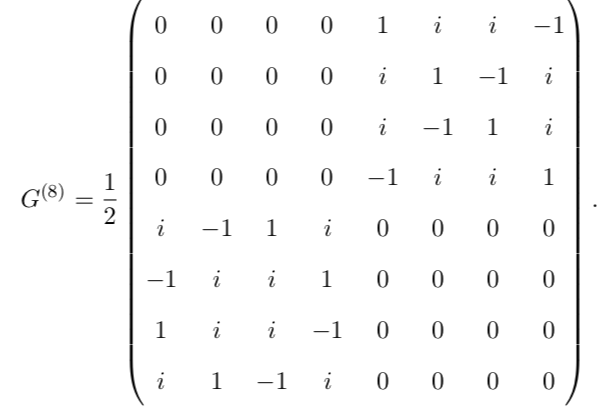
\includegraphics[width = 10cm]{Grover_8.png}$$
This operator is tensor product form of following,
$$G^{(8)} = (H_i \tens{} H_i)\tens{} \sigma_x$$
where, $$H_i = \dfrac{1}{\sqrt{2}}\begin{pmatrix}
           1 & \di\\
           \di & 1
\end{pmatrix}$$

\subsection{Constructing Quantum Circuits}
In this section we will see how to link these universal quantum gates to form a large circuits. Lets take the following circuit diagram,
$$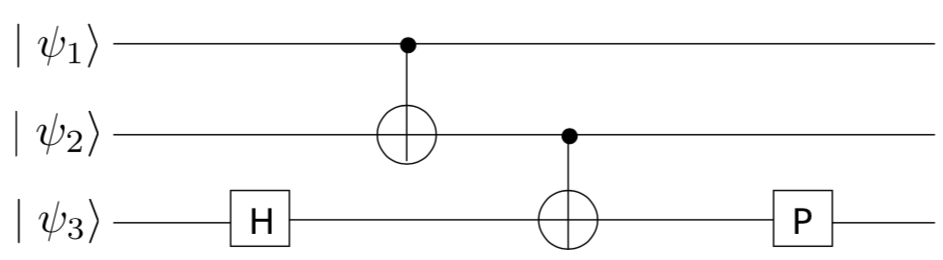
\includegraphics[width = 15cm]{input_circuit.png}$$
For this circuit, we get obtain graph structure by connecting wire and structure so that walk propagates from left to right side. In this, initial state is the left side to the graph with amplitude at each vertex split equally. it is can be think as first column of vertices in superposition. and at the further time steps the subsequent column of vertex can be think as state. so after required number steps, output will be in right side of graph. after construction we get following graph structure,
$$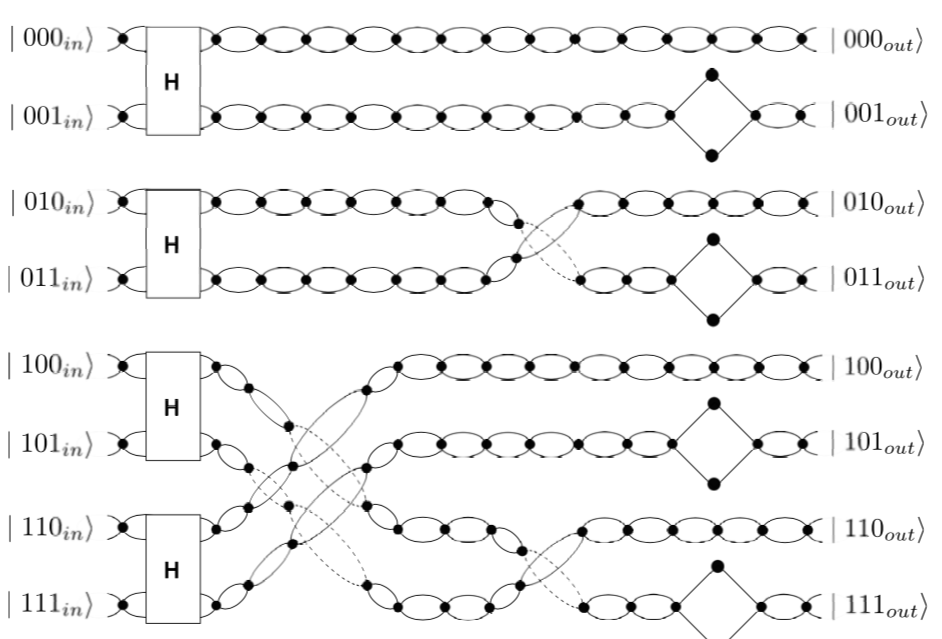
\includegraphics[width =12cm]{graphical_circuit.png}$$
We can see that graph structure is larger than equivalent circuit. As we know, for N qubit computation we need $2^n$ wires which we called basis states.

\section{Discussion}
In this project we described that Discrete time quantum walk can be used as universal computation, it means any quantum algorithm can be recast using discrete time quantum walk. it is different from continuous time walk that also can be used as universal quantum computation as described by [6]Childs.

Although neither continuous nor discrete time quantum walk model for universal computation is designed to implement physically. its only show power of quantum walk algorithms. This all power of quantum walk motivate that many quantum walk algorithm can be found.

\newpage
\section{References}
\begin{enumerate}[label={[\arabic*]}]
    \item Classical and Quantum Computation, A Yu Kitaev, A H Shen, M N Vyalyi(2013)
    \item Quantum computation and quantum information, M.A. Nielsen and Issac L. Chuang (2000).
    \item J. Kempw. Quantum random walk:an introductory overview. Contemp. Phy. 2003
    \item R. Portugal, Quantum walks and search algorithm Springer, 2013
    \item Universal quantum computation using the discrete time quantum walk,Neil B. Lovett, Sally Cooper, Matthew Everitt, Matthew Trevers, Viv Kendon(2010)
    \item Universal computation by quantum walk, Andrew Childs (2009)
    \item Quantum Computing, Jozef Gruska (1999)
    \item Quantum walks: a comprehensive review, Salvador E. Venegas-Andraca(2012)
    \item Quantum Walks, Daniel Reitzner, Daniel Nagaj, Vladimir Buzek (2013)
\end{enumerate}

\end{document}
